\definecolor{lightergray}{RGB}{247,247,247}
\definecolor{darkgreen}{RGB}{36,135,20}
\definecolor{green_comment}{RGB}{0,128,0}
\definecolor{redcell}{RGB}{238,176,176}
\definecolor{greencell}{RGB}{217,234,211}


\chapter{Diseño e Implementaciones}
\label{cap:c3_implementaciones}	


	En este capítulo se presentan los diseños e implementaciones desarrolladas a lo largo del desarrollo del mismo. Empezando con programas sencillos para introducir MPI, y avanzando por nivel de dificultad en los algoritmos de IA. Los algoritmos de clustering son sencillos de entender y de paralelizar. El aprendizaje por refuerzo y los algoritmos evolutivos aumentan la complejidad en las implementaciones y para finalizar las redes neuronales, que de por si tienen un complejidad más elevada.

%\newpage %TODO QUITAR
\section{Programas sencillos}

	Para introducir MPI en el proyecto se implementan y comentan varios programas sencillos. La multiplicación de matrices, que tiene un coste cúbico, al tener que recorrer, para cada elemento de la matriz, una fila y columna entera. Y algoritmos de ordenación, que para simplificar, solo se realizan un estudio de las ordenaciones que más tiempo de ejecución consumen, O(\(N^{2}\)) y MergeSort con coste O(NlogN).


	Las matrices son un concepto matemático muy relevante en el mundo de los videojuegos y en el ámbito de la inteligencia artificial. Hay muchas técnicas de IA que conllevan la gestión de imágenes, como en el algoritmo DQN cuya red neuronal tiene como entrada varios fotogramas para poder aprender. Estas imágenes, pueden en mayor o menor medida ser implementadas con matrices.
	
	El cálculo de la multiplicación de dos matrices es cúbico O(\(N^{3}\)). Recorre toda la matriz, y para cada elemento, hace el sumatorio de las multiplicaciones fila, columna. 
	
	Es un buen primer ejemplo para iniciar con la arquitectura MPI, debido a la lentitud del cálculo. Para ello hay que plantear cómo dividir el trabajo entre los procesos. 
	
	Se puede pensar que es mejor ir enviando los datos conforme se finaliza una operación, pero en esta operación se necesitan las filas de una matriz y columnas de otra, por lo que conviene que cada proceso tenga una matriz entera en su memoria local, para agilizar el proceso y poder enviar más datos al mismo tiempo.


	Cada worker se va a encargar de un determinado número de filas, así paralelizando el cálculo. El master se encarga de dividir la matriz entre los procesos, y se puede abordar con dos enfoques distintos.
	\begin{itemize}
		\item Enviar la división completa de filas a cada worker, y esperar a que terminen todos los cálculos, y el master agrupa los mensajes. 
		\item Ir enviando filas de la matriz conforme se va resolviendo. Así logramos tener un flujo constante de mensajes y reducimos la complejidad espacial.
	\end{itemize}



	\begin{figure}[!h]
		\centering
		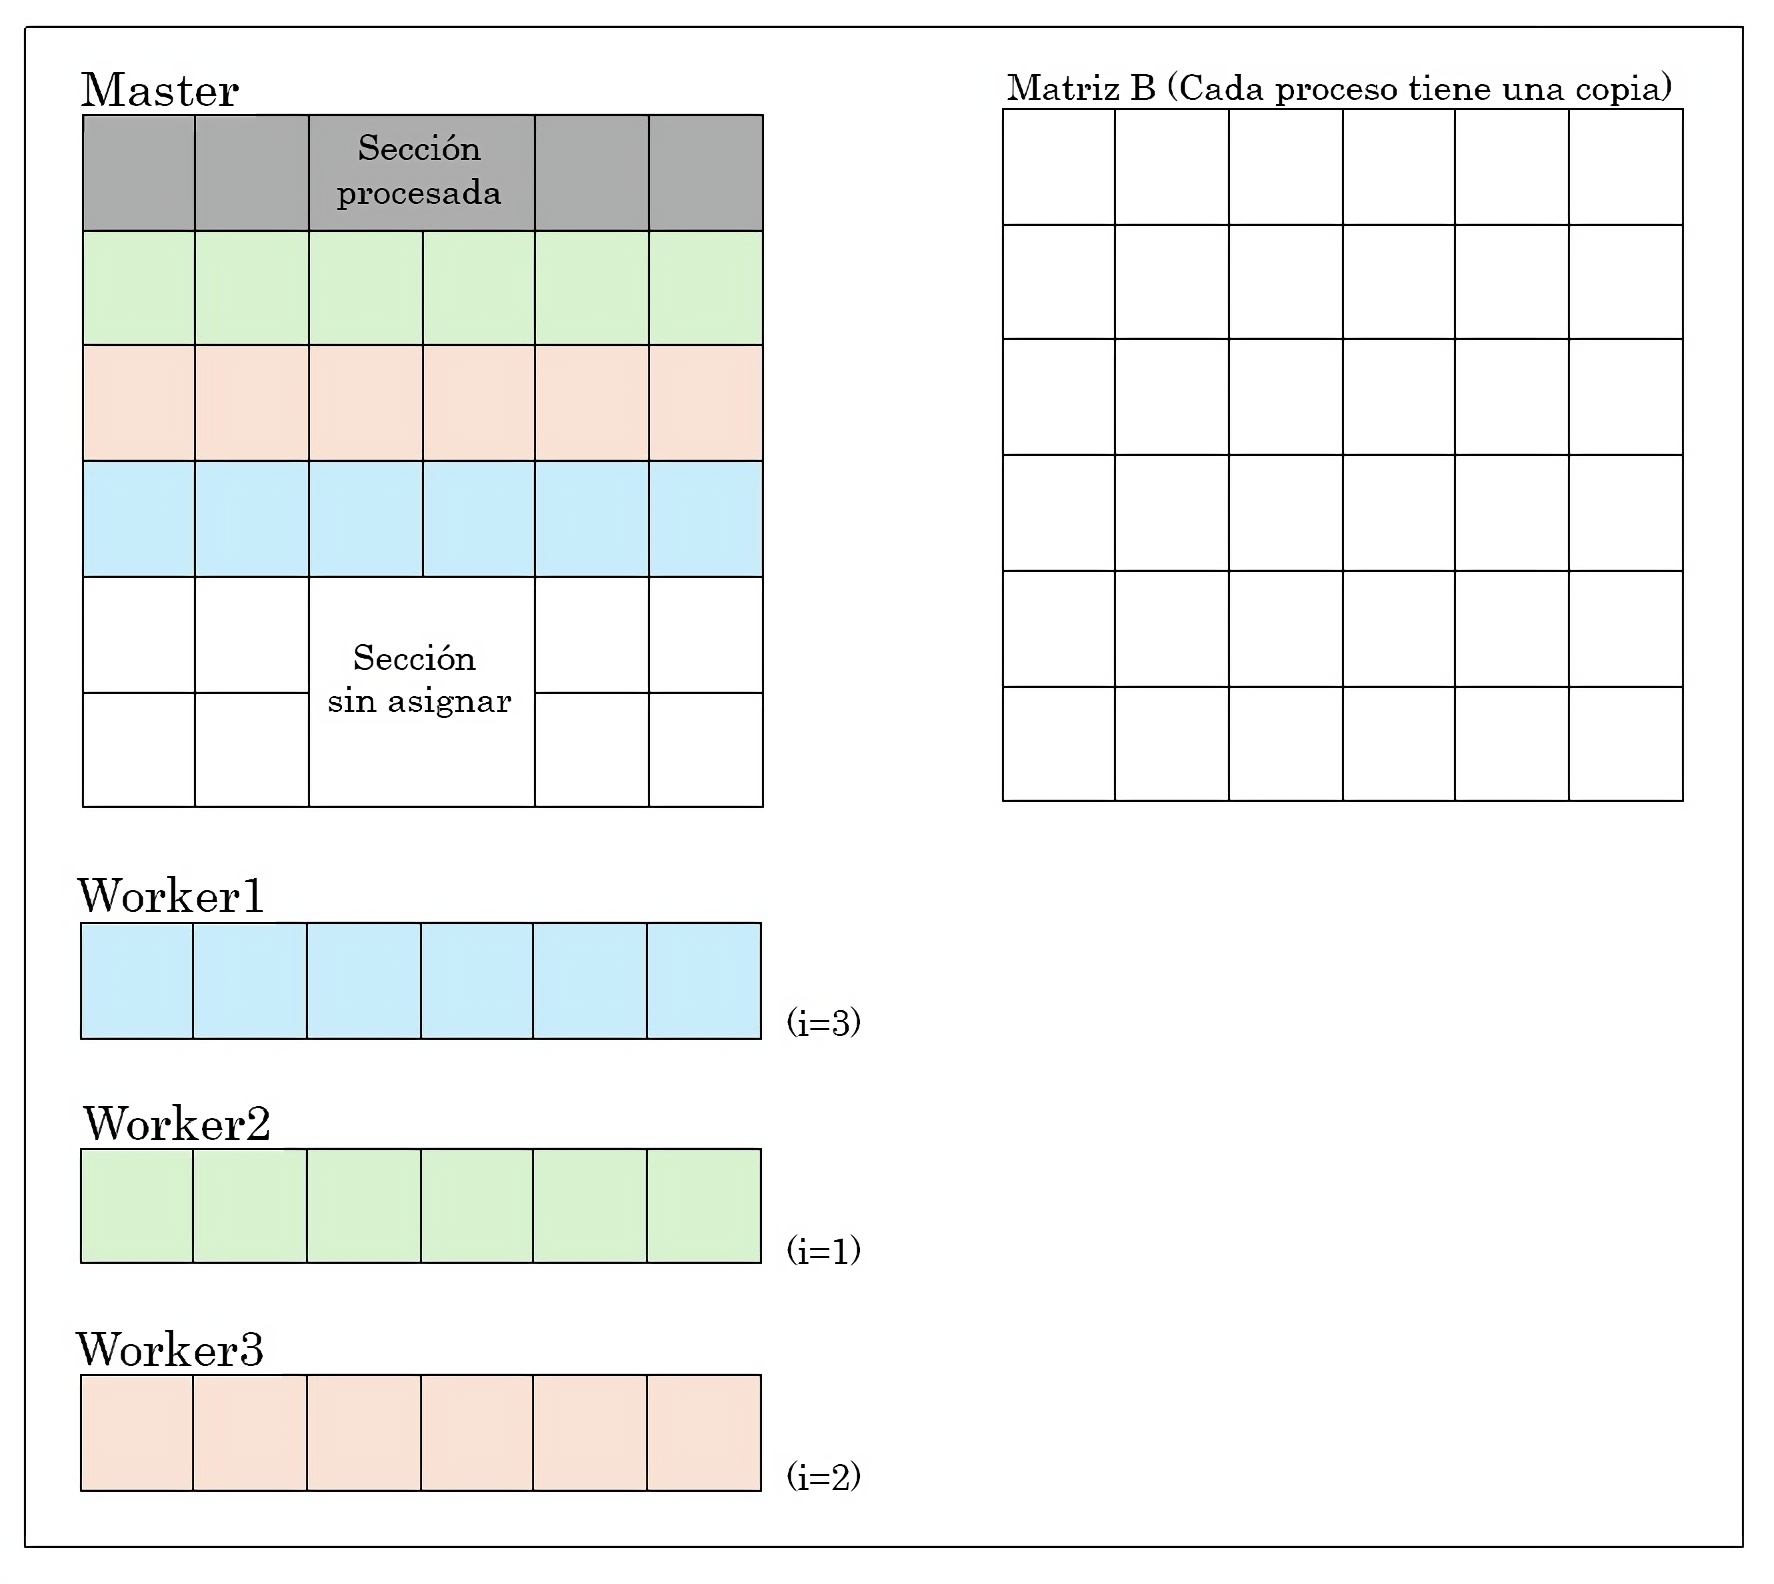
\includegraphics[width=0.58\textwidth]{images/chapter_3/matriz_mpi}
		\caption{MPI - Matriz}
		\label{fig:matrizmpi}
	\end{figure}
	
	En el primer enfoque dejamos al master dormido hasta que recibe los resultados, y al recibir los resultados, se genera un cuello de botella. Además de aumentar la complejidad espacial al tener siempre las filas asignadas. Sin embargo en la segunda idea, el flujo de mensajes hace que el master vaya colocando los resultados recibidos, y se reduce el espacio en memoria, al manejar en cada iteración una fila. Figura \ref{fig:matrizmpi}


	%\vspace*{0.2cm}
	
	
	Los algoritmos de ordenación tienen tienen que iterar varias veces hasta que esté completamente ordenado. Y los métodos pueden variar bastante el tiempo de ejecución.
	
	Para las ordenaciones cuadráticas, los métodos populares son BubbleSort, InsertionSort y SelectionSort, han sido estudiados y optimizados para que aunque tengan un coste cuadrático en el caso peor, tengan un buen rendimiento. Basándome en estos algoritmos he diseñado otro al cual he llamado SequentialSort. Consiste en recorrer todas las posiciones del array, y buscar en qué posición debería de colocarse para que el array esté ordenado. Cada elemento se compara con todos los demás. Se suma uno al contador por cada elemento menor comparado con el actual, y al finalizar una iteración, el contador es la posición del elemento en el array ordenado (si hay repetidos su posición es la primera sin ocupar). Representación en la Figura \ref{fig:sequentialsortmpi} del proceso de ordenación.







	\begin{figure}[!h]
		\centering
		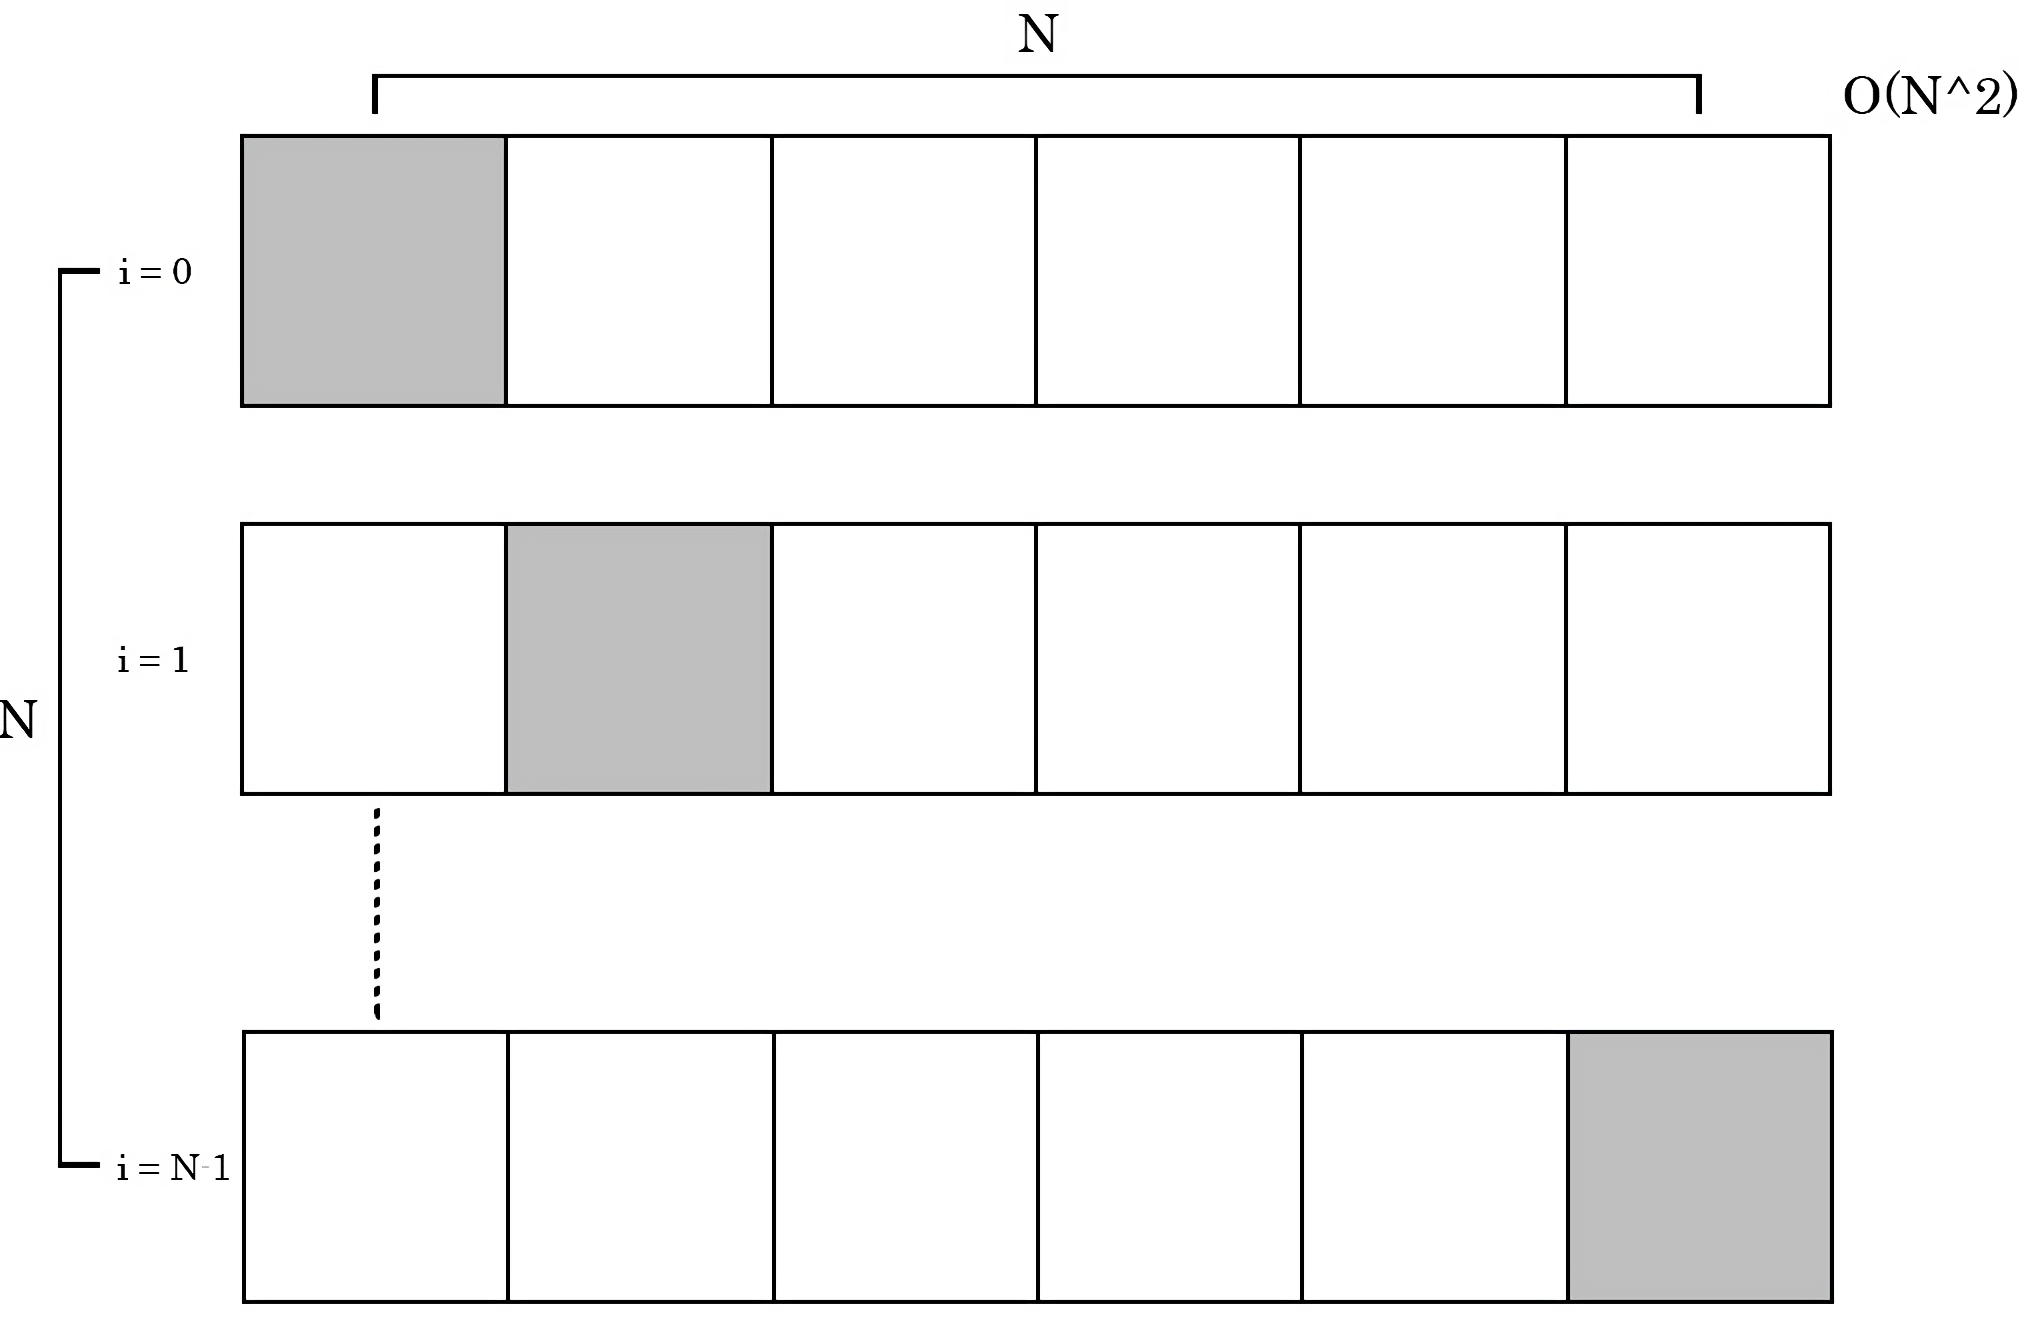
\includegraphics[width=0.6\textwidth]{images/chapter_3/sequentialsort_mpi}
		\caption{MPI - SequentialSort}
		\label{fig:sequentialsortmpi}
	\end{figure}
	
	Este método siempre tendrá coste cuadrático. No es como los anteriores que van reduciendo el espacio conforme aumentan las iteraciones. Pero es fácilmente paralelizable. 
	
	Para lograr esta idea, el master envía a todos los workers el array entero, y además asigna a cada uno qué elementos tiene que buscar su posición en el array ordenado.



	Los algoritmos de ordenación logarítmicos son muy útiles y eficientes. QuickSort tiene varios problemas como la profundidad de recursión y en el caso peor es cuadrático. Los algoritmos de RadixSort y HeapSort son de los mejores si no se aplican mejoras,  y MergeSort es muy popular, tanto que se aplica en Python para el método de ordenación por defecto, TimSort\cite{auger2015merge}. Este último mezcla una ordenación cuadrática optimizada al máximo, para luego usar las mitades ordenadas con MergeSort. Sin embargo, el algoritmo básico de MergeSort no es tan eficiente.
	
	Aplicando la misma idea que TimSort, se puede mejorar el tiempo de ejecución de MergeSort, aplicando combinaciones de los métodos básicos con complejidad cuadrática y comprobar la eficiencia.
	
	
	Aplicando MPI se crean varios procesos (para mayor eficacia y simpleza el número de procesos tiene que ser potencia de dos), y se divide el array entre los procesos.
	\begin{itemize}
		\item Primera fase de ordenación: cada proceso ordena su sub-array con el método de ordenación más eficiente. Una vez desarrollado el estudio, el método básico SelectionSort es el que mejores resultados obtiene.
		\item Segunda fase de reagrupación y ordenación: esta fase se repite hasta solo tener un proceso activo, es decir, el array esté completamente ordenado.
		\item Proceso de comunicación entre procesos. Cada proceso se conecta con el más cercano (activo). 
		El proceso de mayor id manda su array ordenado y finaliza su ejecución. El que recibe se encarga de ordenar ambas mitades en una sola.
	\end{itemize}
	
	
	Se usa barrier MPI, para garantizar que terminen todos al mismo tiempo. Esta mejora aplica la idea de sincronización con barrera simétrica mariposa (Figura \ref{fig:mergesortmpi}). Se espera a los procesos en potencias de dos para sincronizar.  
	
	\begin{figure}[!h]
		\centering
		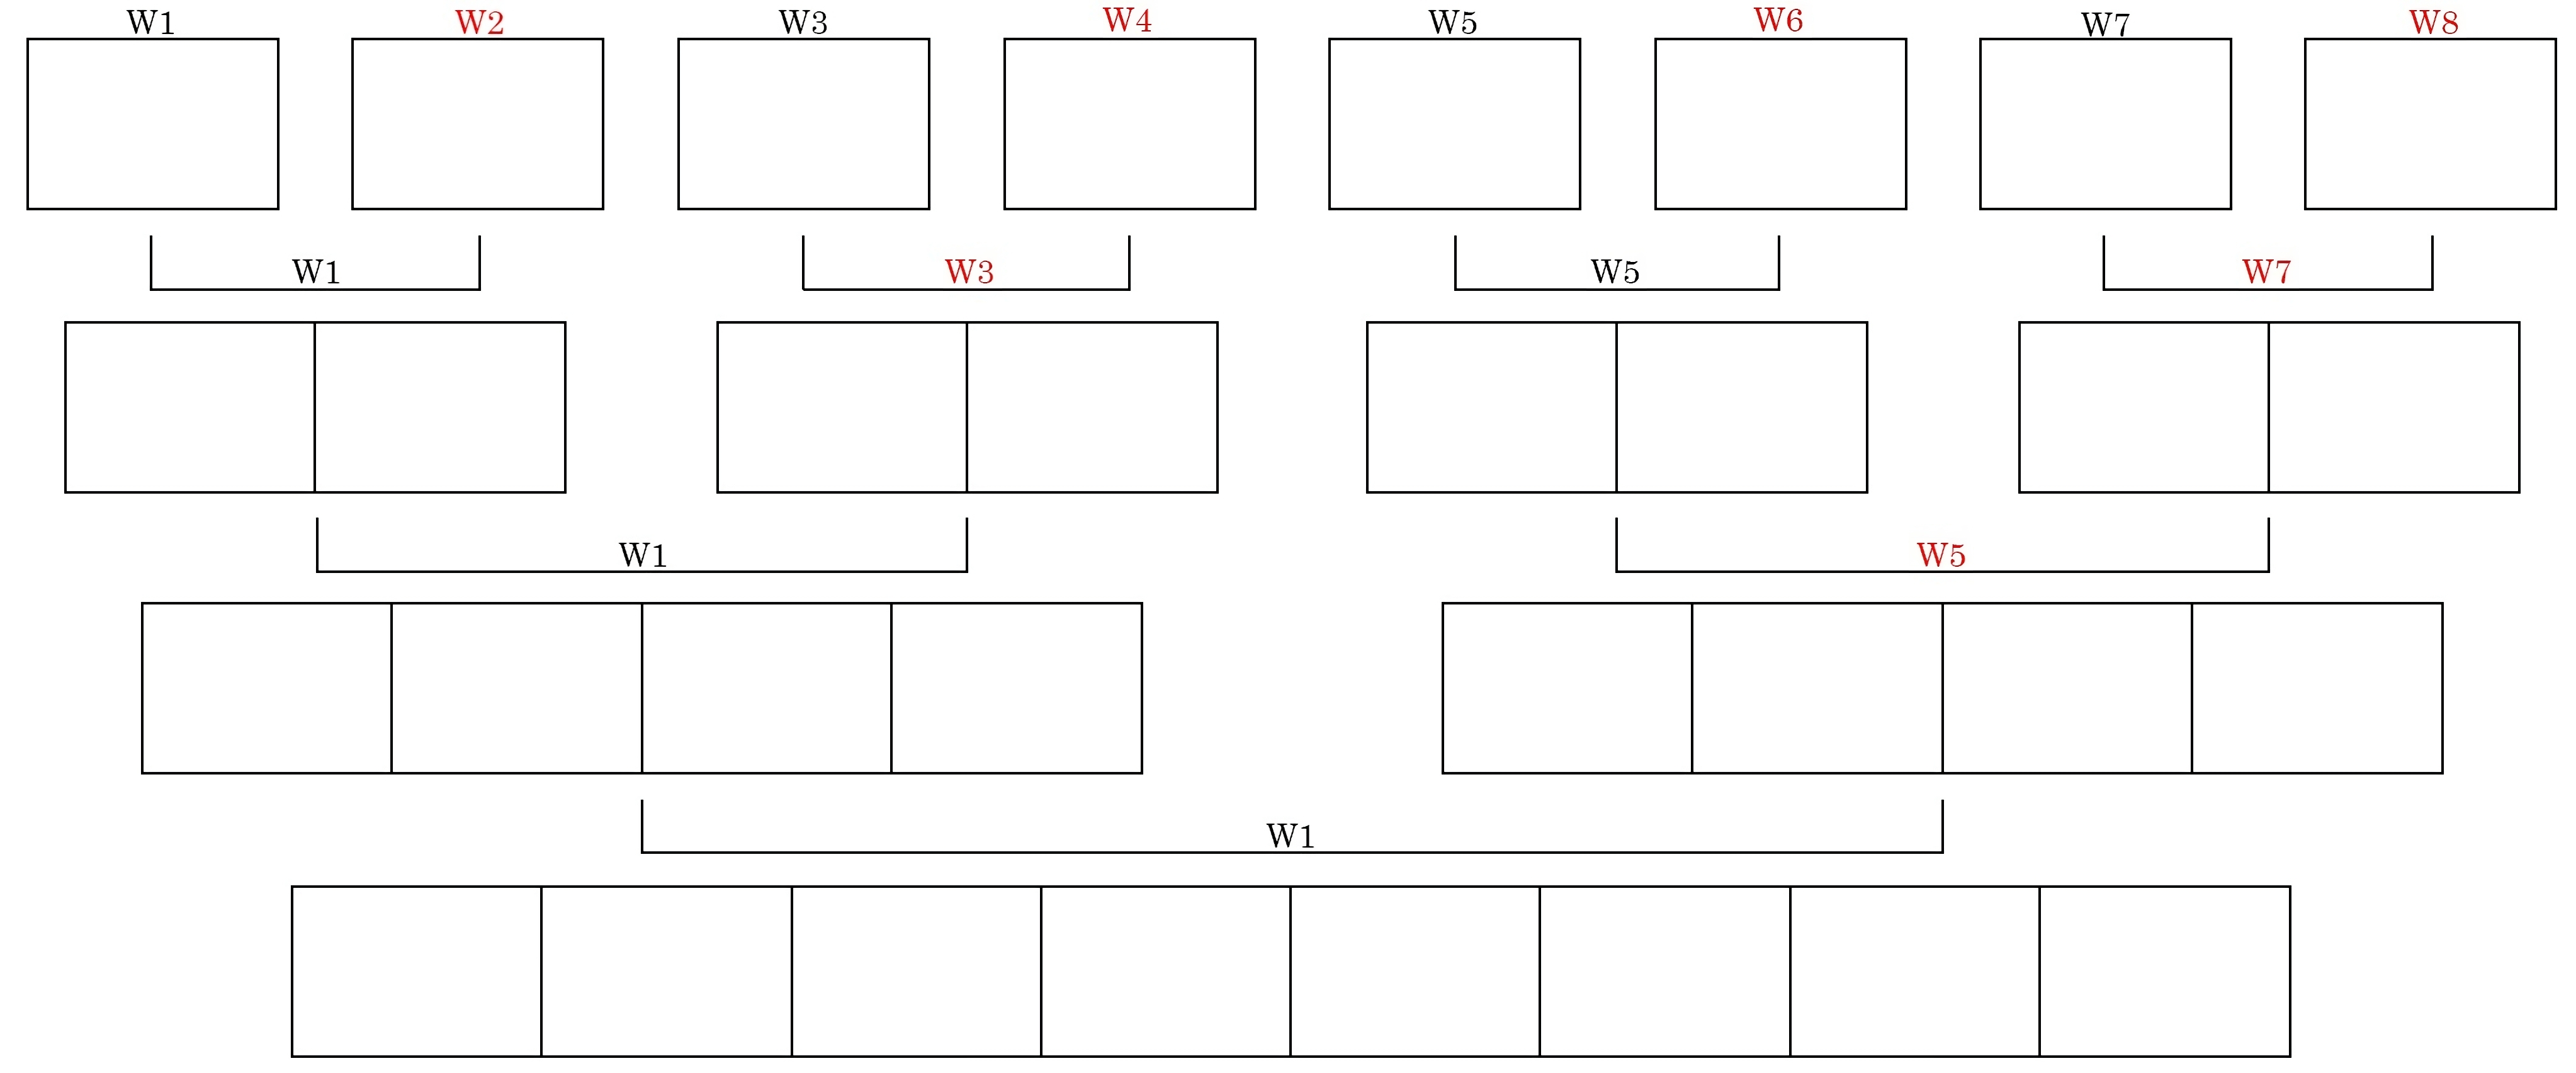
\includegraphics[width=0.65\textwidth]{images/chapter_3/mergesort_mpi}
		\caption{MPI - MergeSort}
		\label{fig:mergesortmpi}
	\end{figure}

	%\begin{figure}[!h]
	%	\centering
	%	
	%	
	%	\begin{subfigure}[t]{0.33\textwidth}
	%		\centering
	%		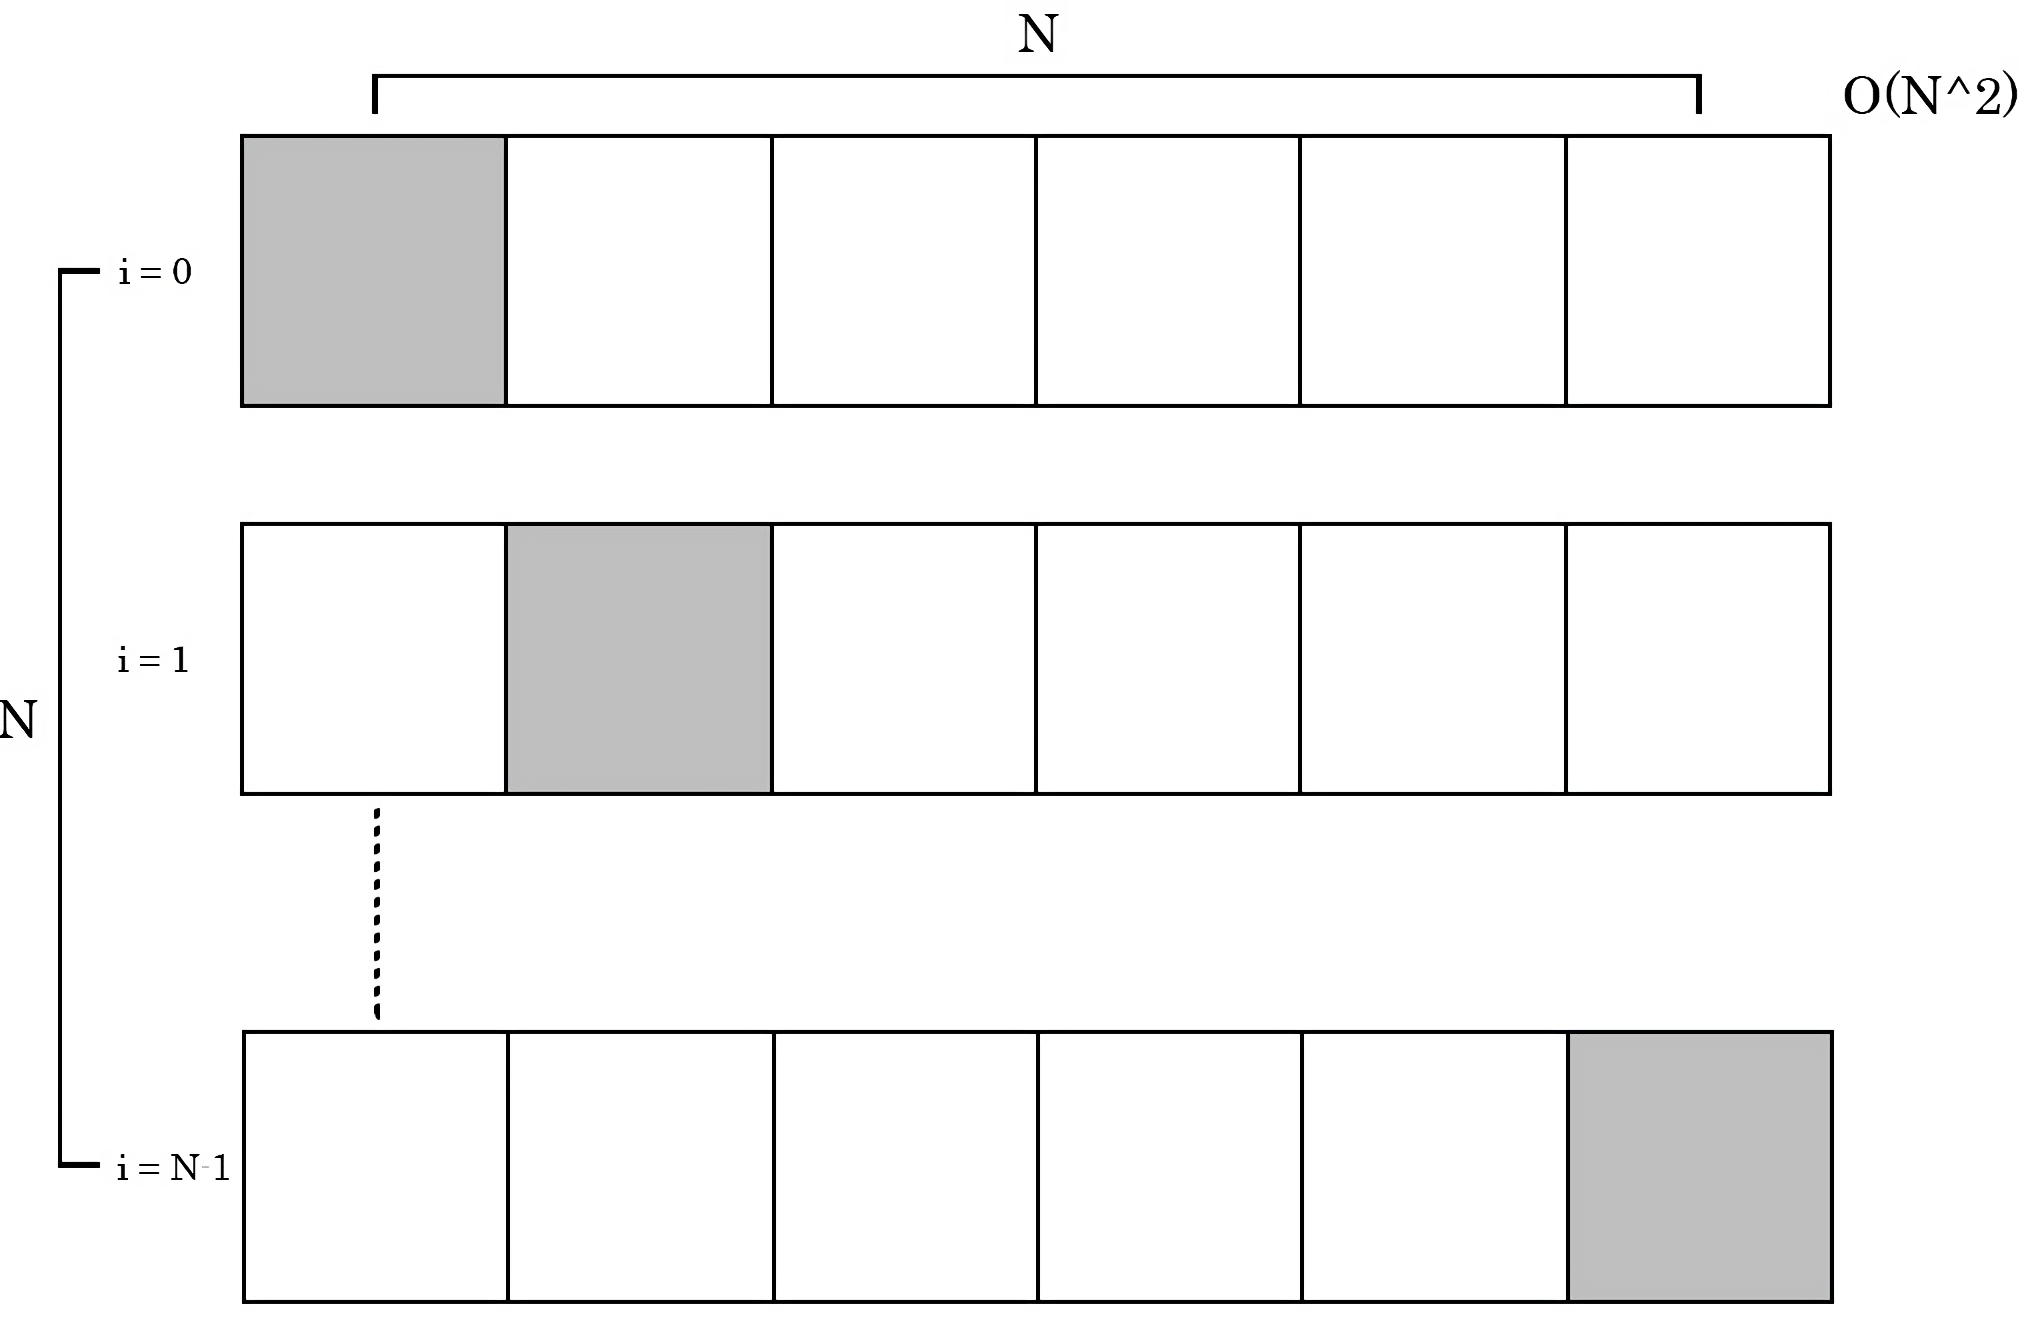
\includegraphics[width=\textwidth]{images/chapter_3/sequentialsort_mpi}
	%		\caption{MPI - SequentialSort}
	%		\label{fig:sequentialsortmpi}
	%	\end{subfigure}
	%	\hfill
	%	\begin{subfigure}[t]{0.48\textwidth}
	%		\centering
	%		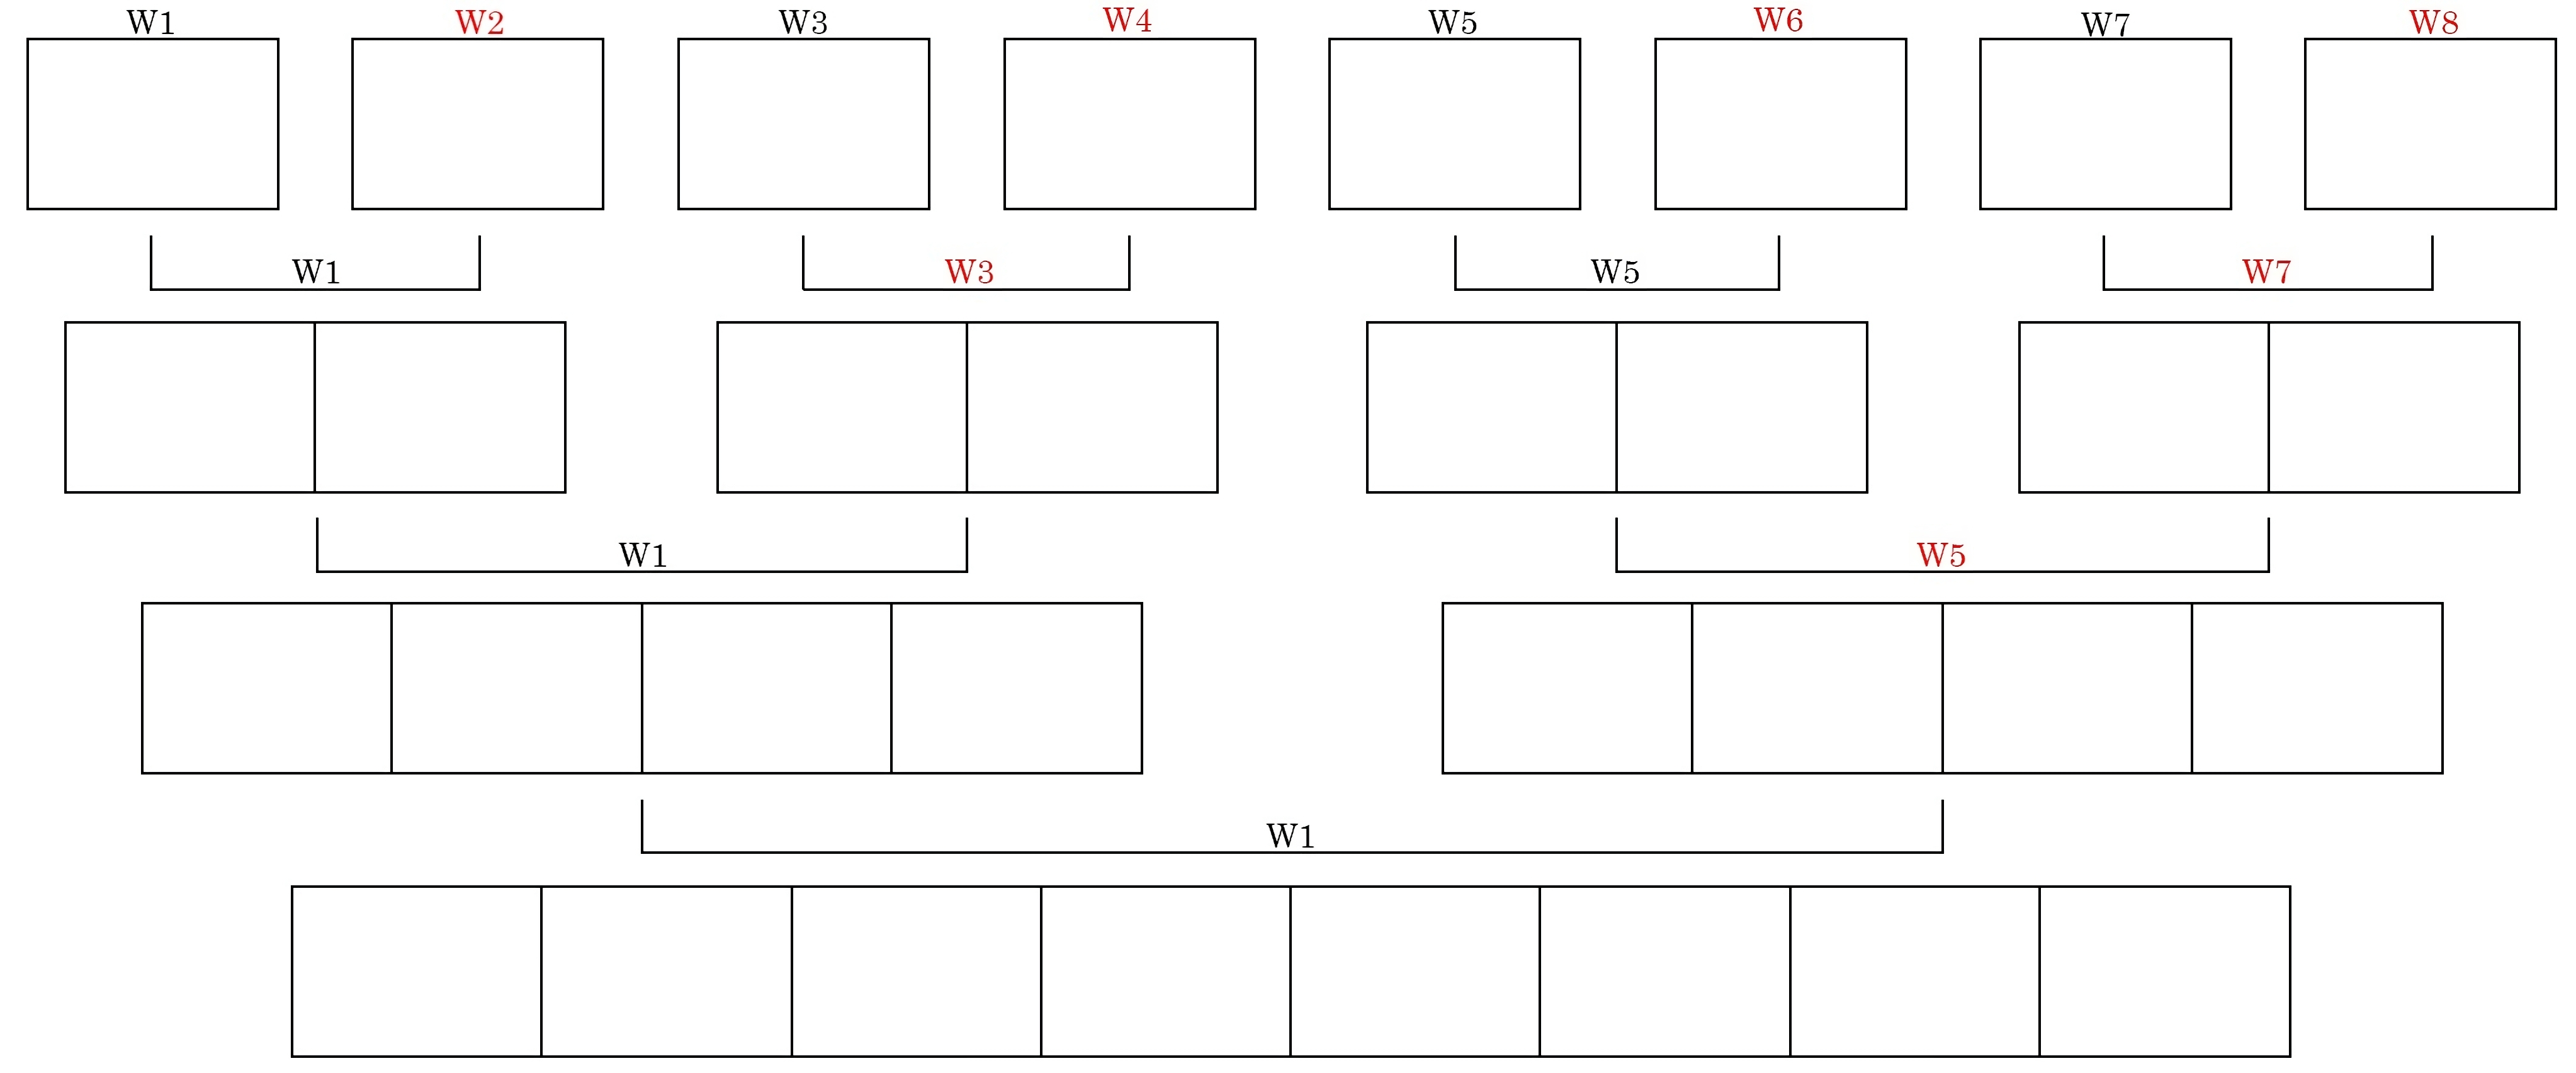
\includegraphics[width=\textwidth]{images/chapter_3/mergesort_mpi}
	%		\caption{MPI - MergeSort}
	%		\label{fig:mergesortmpi}
	%	\end{subfigure}
	%	
	%	\caption{Mejoras MPI de las ordenaciones}
	%	\label{fig:ordenacionesmpi}
	%\end{figure}


	\vspace*{0.2cm}
	
	Para aplicar MPI y paralelizar programas hay que tener en cuenta que la comunicación entre procesos tarda un tiempo. Si queremos reducir el tiempo de ejecución de un programa tenemos que asegurarnos que el programa es viable para paralelizar. Si ejecutamos, por ejemplo una búsqueda lineal en un array, a primera vista, reducir el espacio de búsqueda puede ser beneficioso. Dividiendo el espacio de búsqueda entre los workers reduce el tiempo de O(N) a O(N/numWorkers). Pero ¿se puede reducir el tiempo de ejecución al dividir el espacio entre los workers? 
	
	Hay que tener en cuenta el tiempo de paso de mensajes. Si no se tuviese en cuenta, se podría garantizar la reducción, pero la comunicación entre procesos tiene un coste, y con un tiempo lineal no se pueden lograr mejoras, más bien aumenta el tiempo de búsqueda.
	
	Por este motivo, hay que tener en cuenta la complejidad temporal de los algoritmos que queremos optimizar, porque no siempre es eficiente aplicar paralelismo.

	\newpage 

\section{Algoritmos de Clustering}

	Una vez introducido MPI con programas básicos, podemos pasar empezar a ver las implementaciones de algoritmos relacionados con la inteligencia artificial. La clusterización toma una población, y dependiendo del conjunto de datos categoriza los individuos. Puede ser supervisado, si ademas de la población a categorizar, tenemos un poblacion categorizada previamente. O no-supervisado, si no contamos con esta población etiquetada.

	\subsection{Jerárquico Aglomerativo}
		Este algoritmo usa una matriz para calcular las agrupaciones. Como es una \textbf{matriz simétrica}, podemos reducir la complejidad espacial usando solo el triángulo superior. 
		
		La distancia entre clusters es muy importante. Además de calcular agrupaciones distintas, también varía la complejidad temporal. La más eficaz y rápida es la de centroides, para calcular la distancia entre dos cluster solo necesita el cálculo entre dos puntos (los centros de los clusters). Los demás métodos, enlaces simples y completos, comparan las distancias entre todos los individuos de ambos clusters, provocando un coste mayor. Conviene explotar más el paralelismo en estas distancias.
		
	
		Una vez implementadas las mejoras en el cálculo de multiplicación de matrices, podemos usar estas para mejorar este algoritmo. La primera idea de enviar las filas conforme se realizan los cálculos no se puede aplicar. El algoritmo es más complejo que unos simples sumatorios de multiplicaciones, y varía conforme a la población. Dividir el todo espacio entre los workers esta vez si es óptimo.
		
		Como es una matriz simétrica y se representa con el triángulo superior, hay que dividir la carga de trabajo equitativamente. No podemos implementar una mejora sin dividir el espacio de forma óptima entre los workers. Si dividimos las filas de forma secuencial, el primer worker tendrá muchos más elementos que el último (Figura \ref{fig:JA_distribucion}). 
	
		
		\begin{figure}			
		\begin{mdframed}[roundcorner=5pt]
			\[
			\sum_{i=1}^{\text{filas}} (N - i) \gg \sum_{i=\text{filas}(M-1)}^{\text{filas}(M-1) + \text{filas}} (N - i)
			\]
			\begin{tcolorbox}[boxrule=0.5pt, fontupper=\small]
				
				\textit{N} individuos de la población, \textit{M} procesadores. \textit{N/M} filas para cada worker.\\
				
				Con 100 individuos de población y 4 workers, cada uno tendrá 25 filas. Por lo que:\\
				Worker1 tiene las filas de 1-25, con 2175 elementos. \\
				Worker4, las filas de 76-100, con solo 300 elementos. \\
				El Worker1 tiene 7.25 veces más elementos, no reducirá el tiempo de ejecución.
							
			\end{tcolorbox}
			
		\end{mdframed}
		\label{fig:JA_distribucion}
		\caption{Jerarquico Aglomerativo - Cálculo de la distribución óptima}
		\end{figure}
		
		
		Dividiendo las filas por pares (parte superior, parte inferior) repartimos de forma óptima las filas para cada worker. Figura \ref{fig:aglomerativompi}.
		
		Así cada worker tiene el mismo número de elementos que calcular y analizar, inicialmente. 
		
		\begin{figure}[!h]
			\centering
			
			
			\begin{subfigure}[t]{0.4\textwidth}
				\centering
				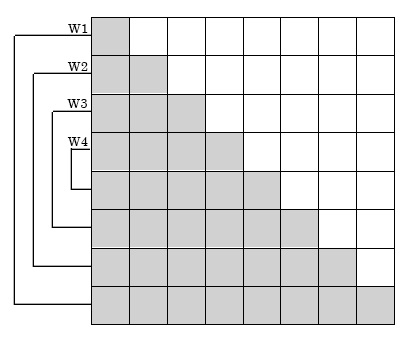
\includegraphics[width=\textwidth]{images/chapter_3/aglomerativo_mpi}
				\caption{División óptima}
				\label{fig:aglomerativompi}
			\end{subfigure}
			\hfill
			\begin{subfigure}[t]{0.52\textwidth}
				\centering
				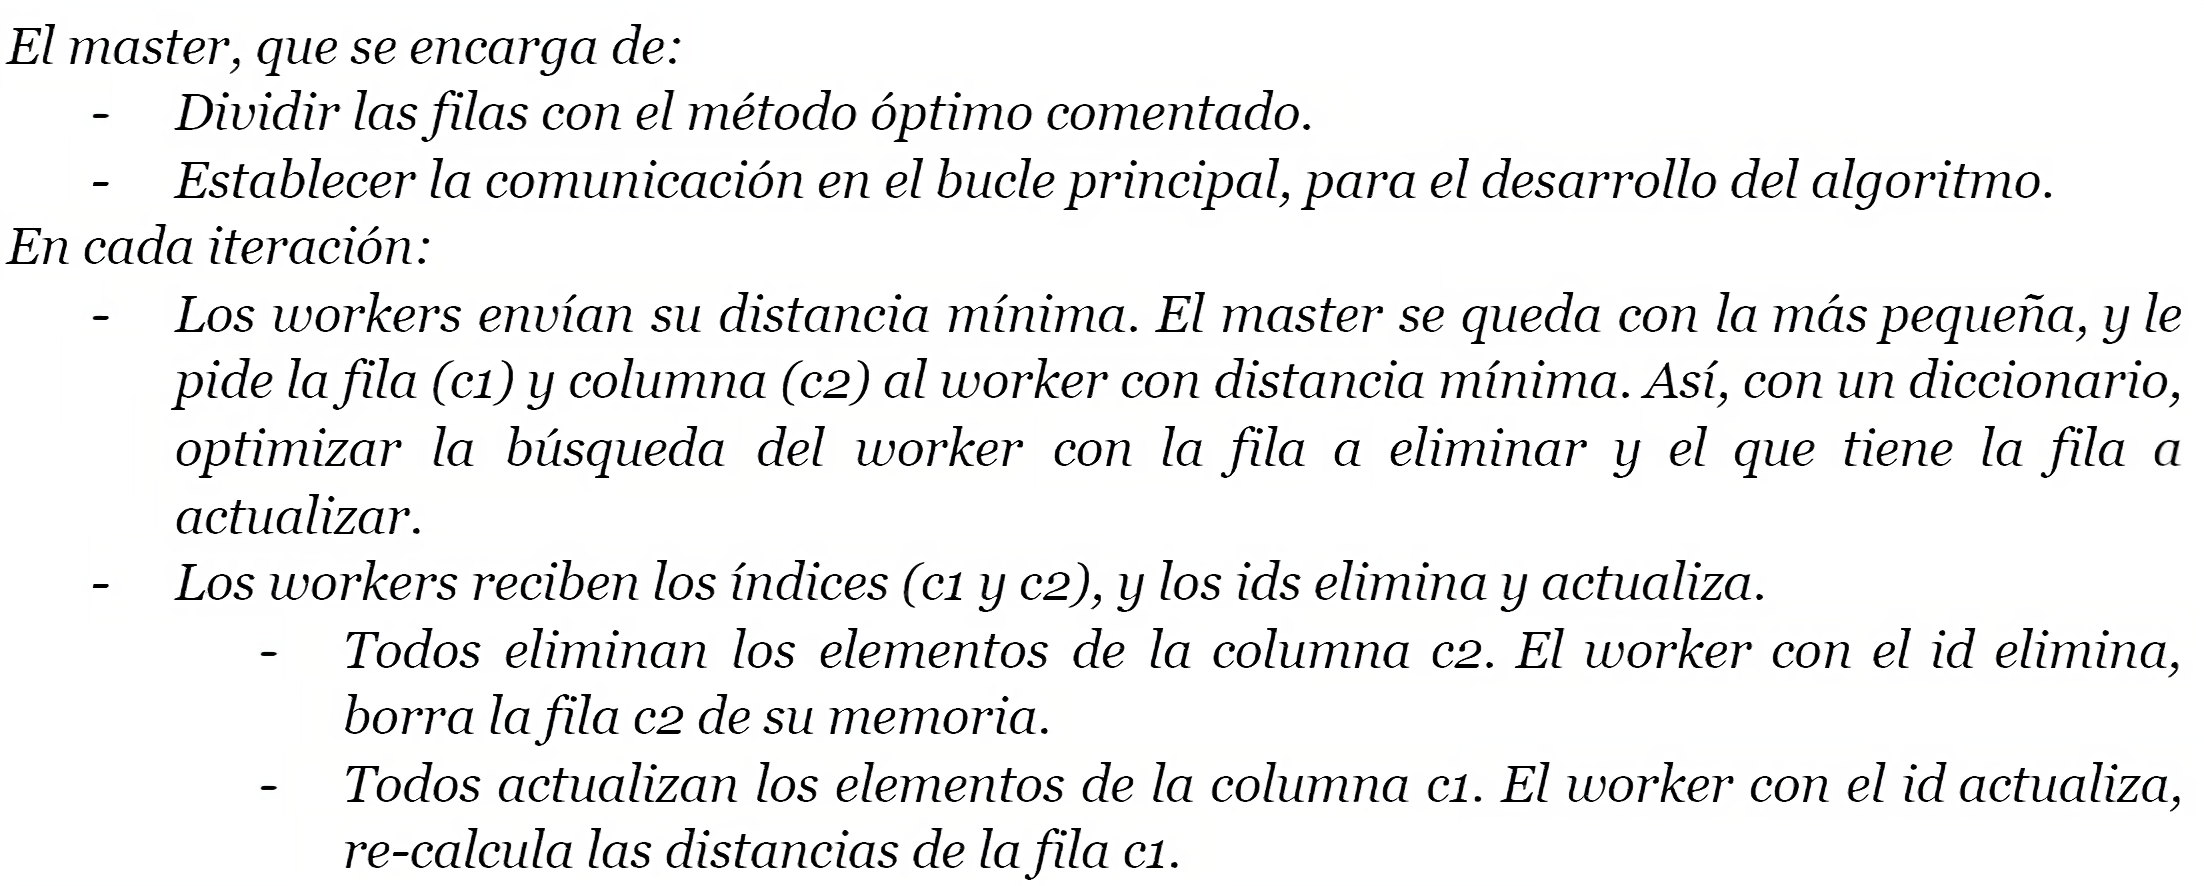
\includegraphics[width=\textwidth,height=5cm]{images/chapter_3/aglomerativo_sec}
				\caption{Tareas de los proceso}
				\label{fig:aglomerativosec}
			\end{subfigure}
			
			\caption{MPI - Jerarquico Aglomerativo}
			\label{fig:aglomerativo}
		\end{figure}
		
		
		Una vez descrito el reparto de espacio entre los procesos, cada uno tiene que ejecutar el algoritmo en paralelo, sincronizandose cada cierto tiempo para actualizar valores.
		
		Refrescando la memoria, este algoritmo en cada iteración agrupa los dos individuos más cercanos. Eliminando una fila y columna de la matriz.
		
		\newpage
		
			
	
			
			
			
			
		
		El cálculo de las distancias de la nueva fila usando distancias de centroides es lineal, no se puede reducir el tiempo de ejecución. Pero para los enlaces simples y completos, que tienen un coste cuadrático, se debe intentar reducir el tiempo de cómputo. Para lograrlo se puede dividir el cálculo entre todos los workers. 
		
		Hay que encontrar una manera óptima de realizar el cálculo. 
		\begin{itemize}
			\item Cuando hay pocos individuos por cluster, es más probable que haya muchas columnas que actualizar, y conviene dividir el cálculo de distancias de todas las celdas. 
			\item Sin embargo, cuando aumentan los individuos, reducen las columnas y esta idea ya no conviene. Cada proceso estaría mucho tiempo realizando los cálculos. Por eso es mejor ir calculando las distancias de forma escalonada usando todos los worker, dividiendo los individuos del cluster para encontrar la distancia mínima (simple) o máxima (completa).
		\end{itemize}
		
		
		
		
	\subsection{K-Medias}
		Perteneciente al aprendizaje no supervisado, es una técnica de clustering en la cual tenemos una población inicial de individuos sin clasificar, y un valor K sujeto a una asignación flexible según nuestros criterios. Al contrario al algoritmo anterior no se usa una matriz, y solo se usa distancia por centroides. Una mejora MPI se puede implementar de las siguientes formas:
		
		\begin{flushleft}
			1. Dividir la población entre los workers. Figura \ref{fig:kmediasdiv} \\
			2. Ir repartiendo partes de la población para que se vayan procesando y enviando.\\
		\end{flushleft}
		
		La primera idea es la más simple y la que mejor suena en un primer momento. El master se encarga de generar los centroides de manera aleatoria, eligiendo K individuos al azar, sin repeticiones. Mediante broadcast los workers reciben estos centros, y con conexiones punto-a-punto se recibe la población dividida sin intersecciones. Cada worker se encarga de una subpoblación. 
		
		
		
		\begin{mdframed}[roundcorner=5pt]
			El siguiente proceso se repite hasta que el master envie un mensaje de finalización, es decir, no cambien los centros:	
			\begin{itemize}
				\setlength\itemsep{0em} % Ajusta el espaciado entre los ítems
				\item Los workers calculan la asignación de sus individuos. Además calculan la suma de distancias de los individuos a sus centros y el número de individuos asociado a cada cluster. Estos valores los envían al master.
				\item El master recibe estos valores y calcula los nuevos centroides. Manda un mensaje a todos los workers. 
				\begin{itemize}
					\setlength\itemsep{0em} % Ajusta el espaciado entre los ítems
					\item CentroidesNuevos, si los centros cambian. Se actualizan los centros.
					\item Finalización, en caso contrario.
				\end{itemize}
			\end{itemize}
		\end{mdframed}
		
	
		
		Después de ver e implementar la primera opción, no es una buena idea tener un flujo constante de mensajes, pidiendo nuevos datos. La población no cambia, solo cambia la asignación de los individuos y los centros de los clusters. Solo es necesario un mensaje para recibir la población.
		
		
		\begin{figure}
			\centering
			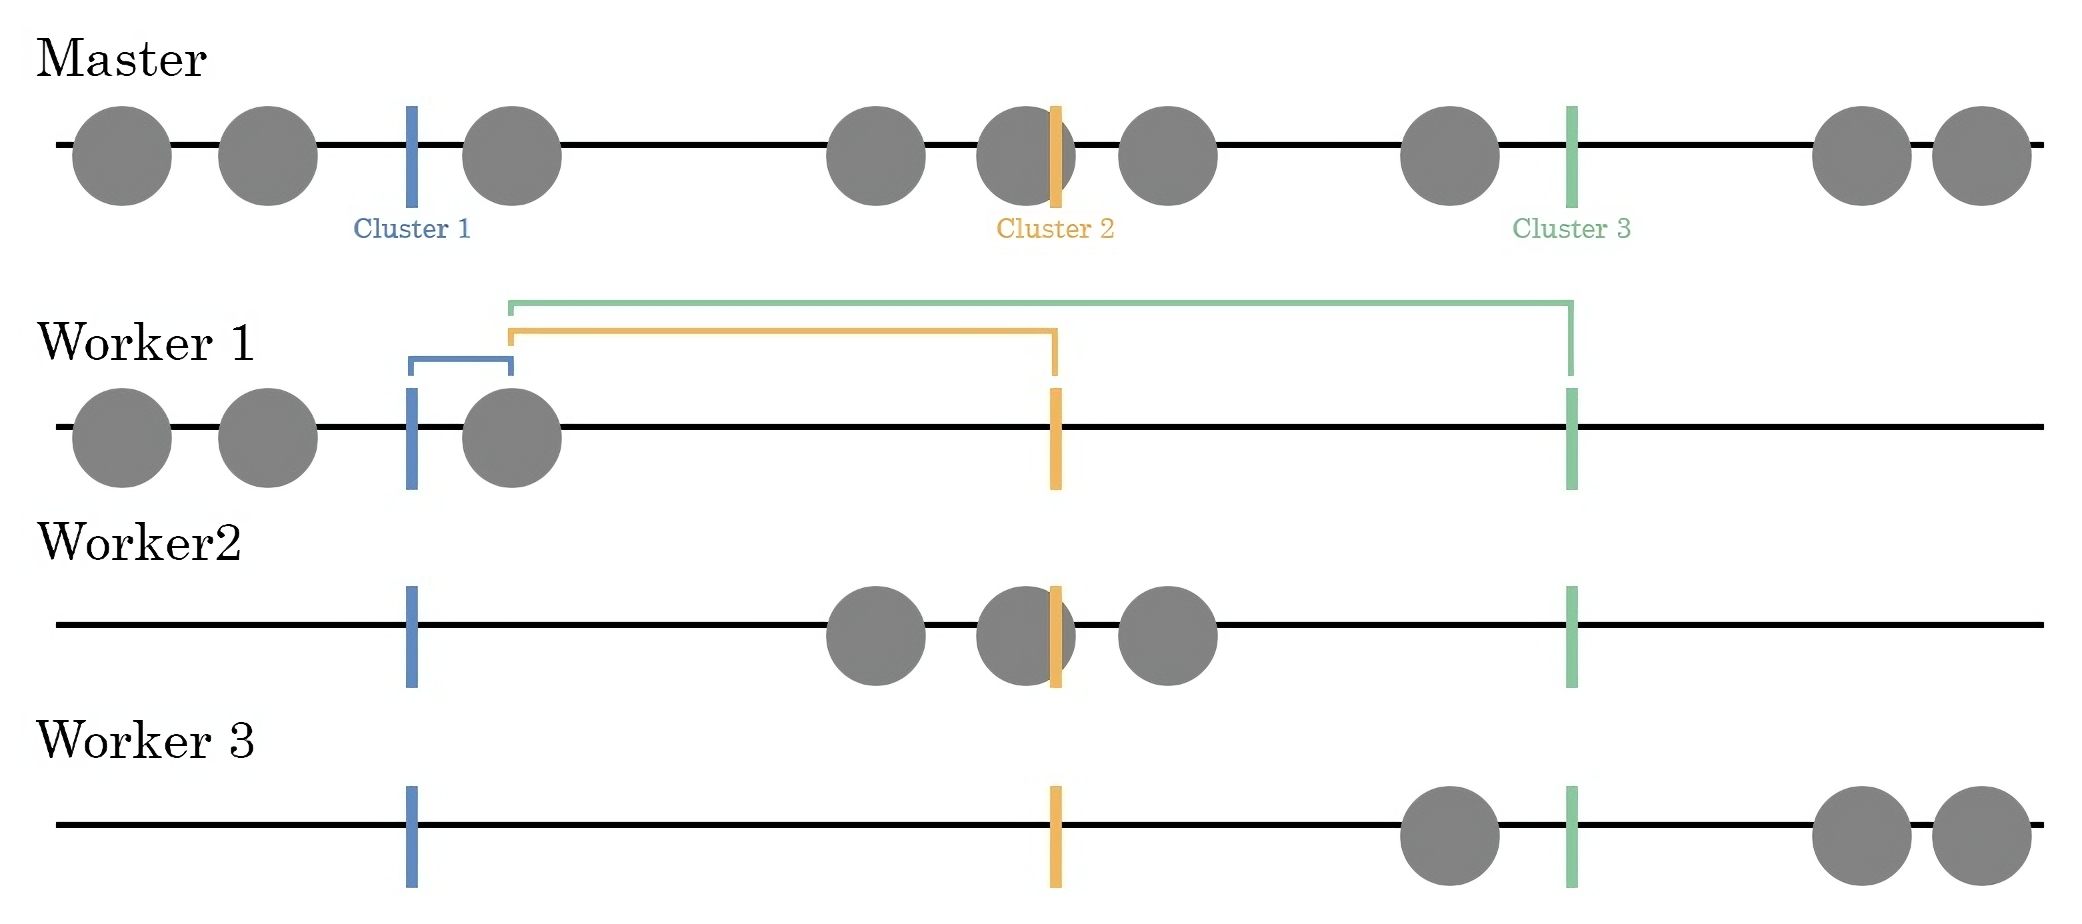
\includegraphics[width=0.8\textwidth]{images/chapter_3/kmedias_mpi}	
			\caption{KMedias - División de poblaciones}
			\label{fig:kmediasdiv}
		\end{figure}
		
		\vspace{0.2cm}
		
		\noindent Búsqueda del óptimo general, y mejor valor para K.\\
		Si queremos realizar este proceso, vamos a necesitar ejecutar la búsqueda del óptimo general para ciertos valores de K. Por lo que se van a necesitar muchas ejecuciones del algoritmo.
		
		\begin{flushleft}
			1. Se puede aplicar la técnica mejorada MPI, con dos bucles. El más externo varía los valores para K, y el interno ejecuta varias veces el algoritmo para conseguir la mejor asignación.\\
			2. Cada proceso ejecuta la búsqueda del óptimo general para valores de K distintos. El master se encarga de recibir las mejores asignaciones y calcular el mejor valor para K, aplicando coeficientes de optimalidad. Esta idea tiene un coste mucho mayor, puesto que cada proceso tendrá la población entera.
		\end{flushleft}
		
		\begin{figure}
			\begin{mdframed}[roundcorner=5pt]
				\[
				O((T \times (N \times K)) \times \text{Rep} \times K_{\text{max}}) \approx O\left(\frac{{(T \times (N \times K)) \times \text{Rep} \times K_{\text{max}}}}{{M}}\right)
				\]
				
				
				\begin{tcolorbox}[boxrule=0.5pt, fontupper=\small]
					
					\textit{T} = número de iteraciones en el algoritmo de K-Medias\\
					\textit{N} = número de individuos en la población\\
					\textit{M} = número de proceso\\
					\textit{Rep = }repeticiones para buscar el óptimo general\\
					\textit{KMax} = valor máximo de K en la búsqueda.				
					
				\end{tcolorbox}
				
			\end{mdframed}
			\caption{KMedias - Comparación temporal de las mejoras}
			\label{fig:KMedias_comp}
		\end{figure}
		
		Ambas ideas tienen el mismo coste temporal, sin contar los mensajes en MPI. Pero la segunda opción tiene un coste espacial mayor, por lo que reduce la eficiencia al crear muchos procesos.
		
		
	\subsection{K-Vecinos más cercanos (KNN)}
		Tenemos un valor K  asignado de manera arbitraria como en el algoritmo de K-Medias. Esta técnica de clustering pertenece al aprendizaje supervisado, tenemos una población de individuos categorizados con las etiquetas de asignacion de cluster. Y una población a predecir.
		
		Aplicando una cola de prioridad de máximos para el cálculo de los K vecinos más cercanos, reducimos la complejidad del algoritmo. Al recorrer la población categorizada, se compara con la cima de la cola. Si la distancia a comparar es menor que la cima, se elimina la cima y se introduce la nueva distancia. Los valores de la cola se mueven con la restricción de prioridad. Y al finalizar la búsqueda en la población se cuentan los elementos de la cola, para saber qué cluster se repite más.
		
		Es importante actualizar la población conforme se van prediciendo los valores, para tener más puntos de referencia. Si no actualizamos la población, la agrupación de los individuos puede variar mucho. Aunque es menos precisa a la hora de predecir, el algoritmo es más veloz, al no aumentar la población categorizada. Al tener una población extra (la categorizada) hay dos formas de implementación posible:
		
		
		\begin{flushleft}
			1. Dividir la población categorizada entre los workers. (Figura \ref{fig:knn1})\\
			2. Dividir la población a predecir entre los workers. (Figura \ref{fig:knn2})
		\end{flushleft}
		
		Si dividimos la población categorizada (primera idea), los workers trabajan menos en cada individuo. Comparan el individuo a predecir con su subpoblación, y el master trabaja más, al recibir los K vecinos de cada worker.  Mientras que el master comprueba las distancias recibidas, los workers trabajan con el siguiente valor a predecir. Para la actualización de individuos, el master reparte de forma equitativa. En cada iteración envía el individuo categorizado a uno distinto.
		
		Con la división de la población a predecir (segunda idea), cada worker trabaja lo mismo, pero predice menos individuos. El máster no trabaja tanto como en la mejora anterior, solo recibe la categorización de los workers. Actualizar la población se puede realizar de varias formas, ya que aquí todos los workers comparten la población categorizada, no como en el anterior. Se puede hacer enviando M nuevos individuos a los M workers ejecutados, en cada iteración, es decir, al recibir un individuo predicho de cada worker. O cada X iteracioens, enviar los nuevos individuos categorizados.
		

		\begin{flushleft}
			El coste espacial depende de los tamaños de las poblaciones.		
		\end{flushleft}
		
		\begin{itemize}
			\item La primera idea, al dividir la población inicial, es más eficiente cuando esta población inicial es mayor a la de predicción. 
			\item En su contraparte, la segunda implementación, al dividir la población a predecir, tiene un mejor rendimiento con poblaciones de predicción mayores.
		\end{itemize}
		
		\begin{figure}[!h]
			\centering
			
			
			\begin{subfigure}[t]{0.45\textwidth}
				\centering
				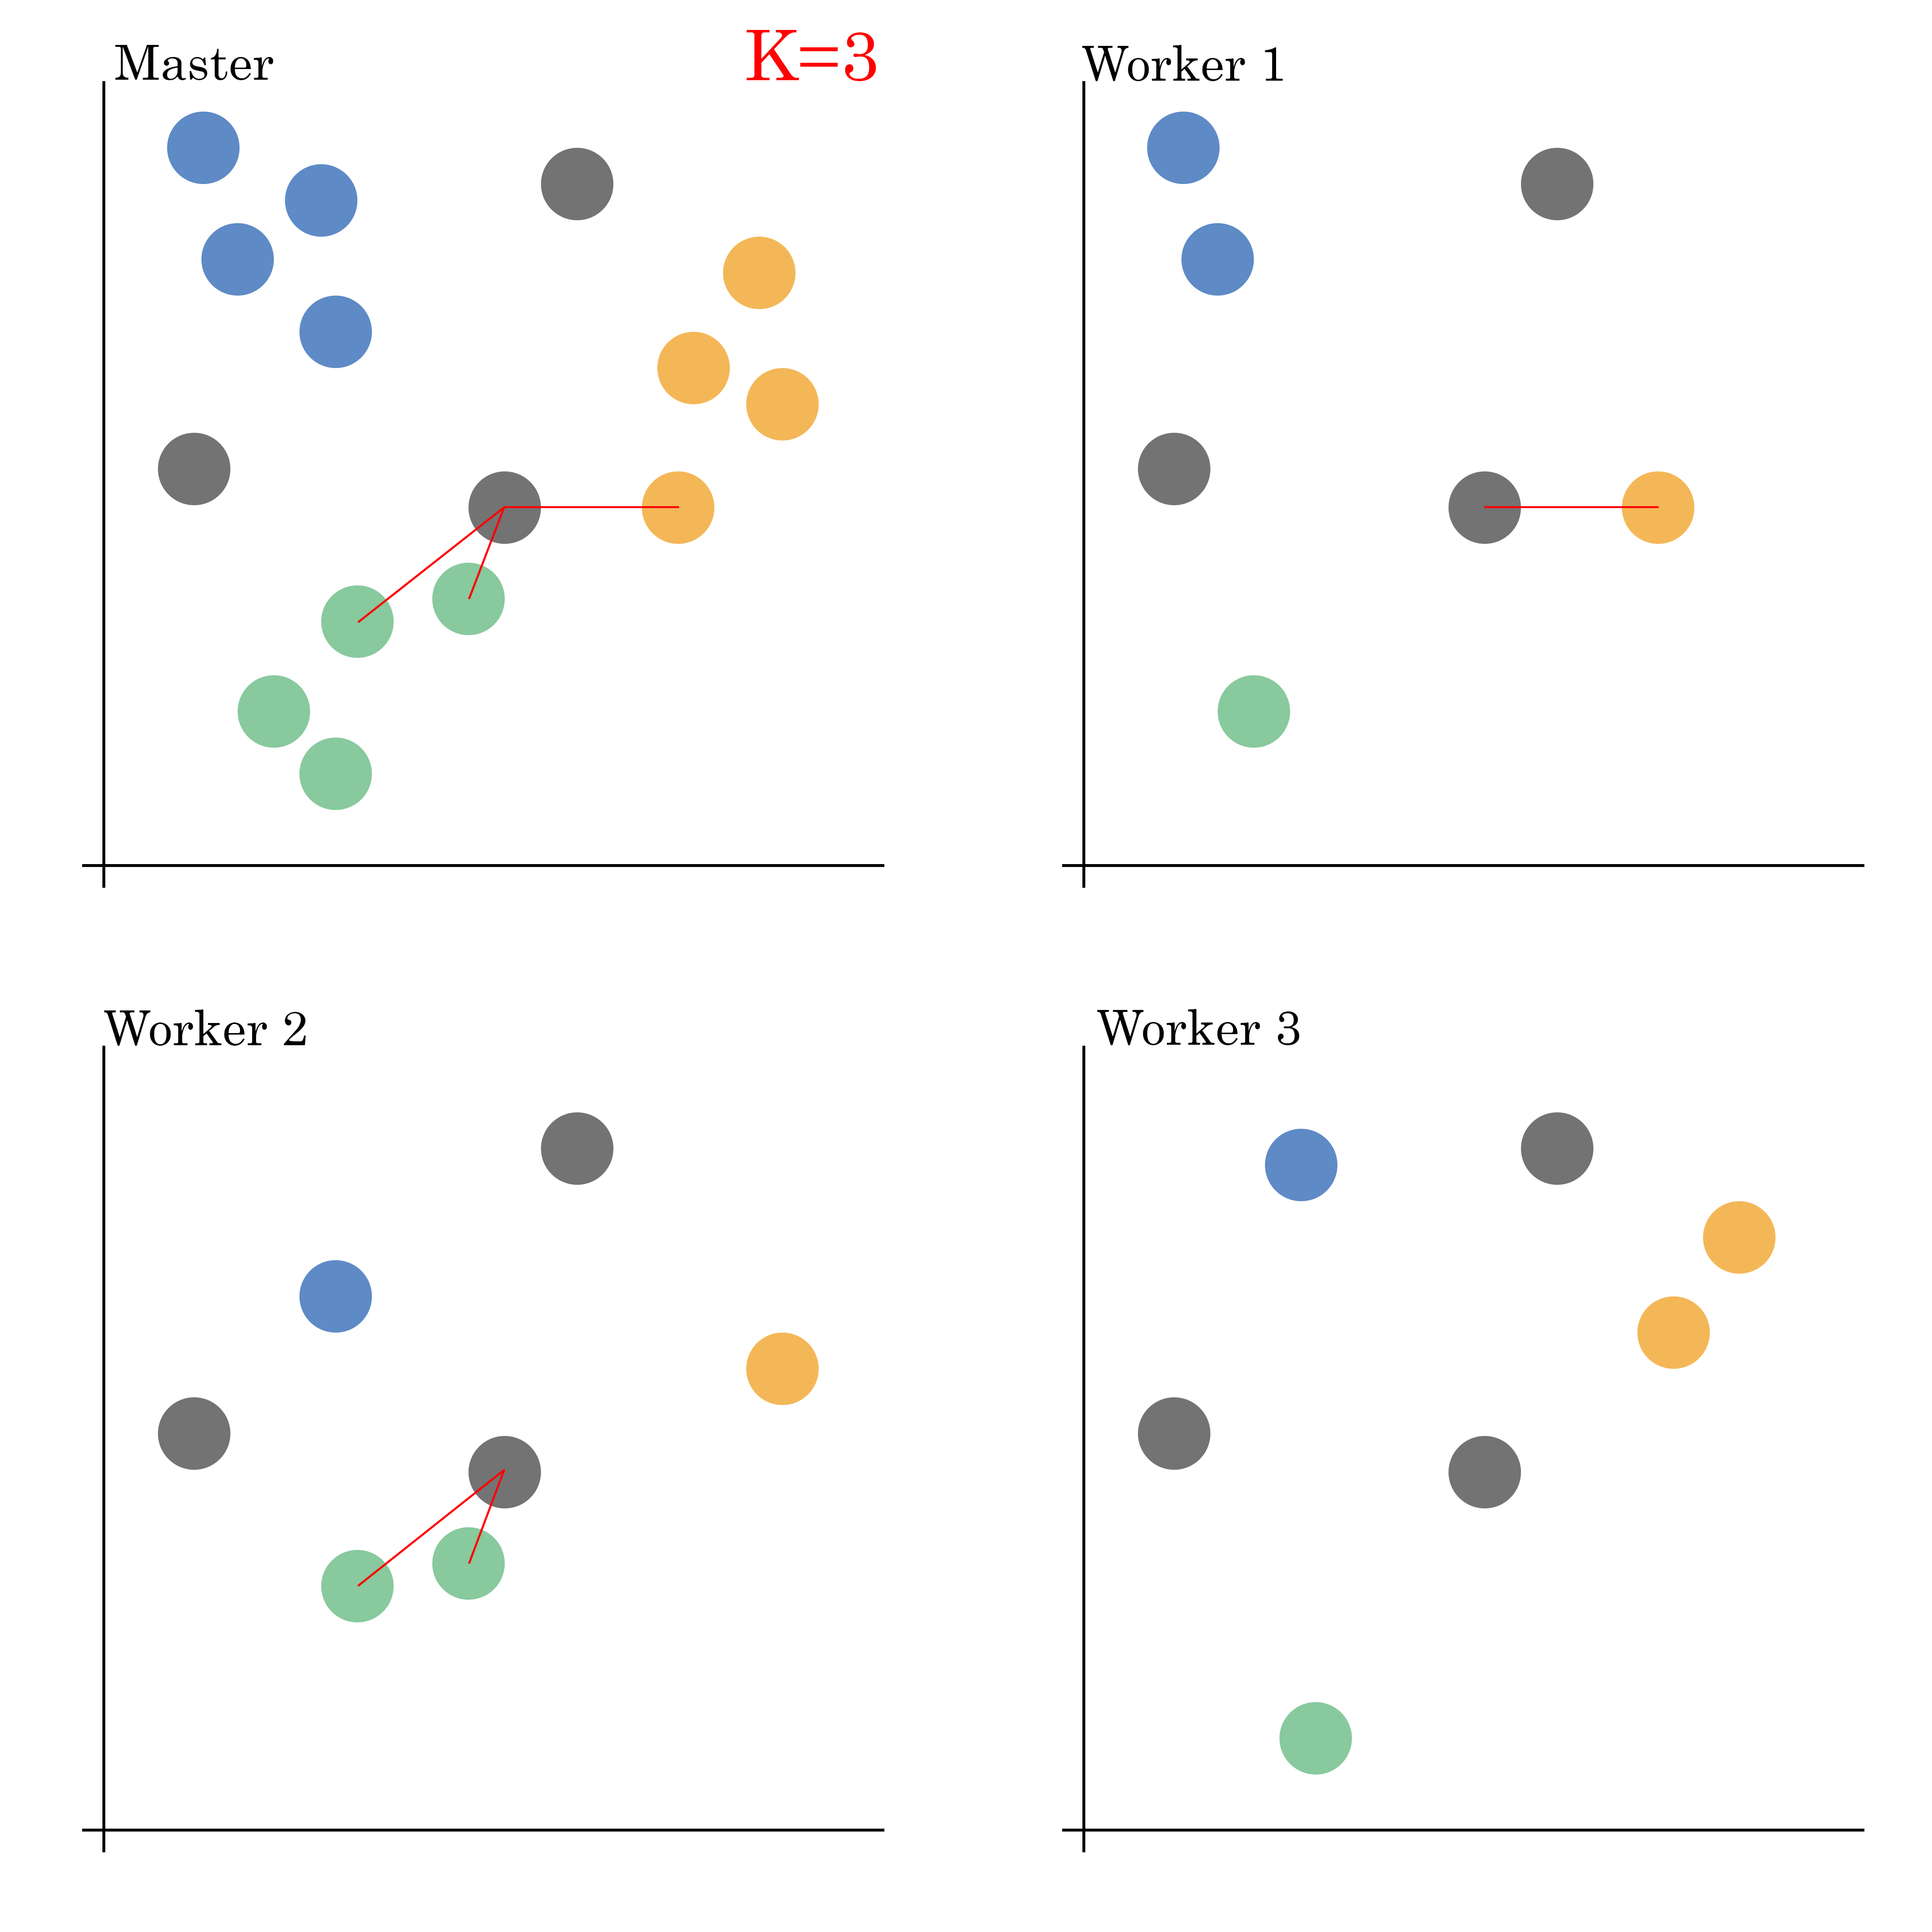
\includegraphics[width=\textwidth]{images/chapter_3/knn_mpi1}
				\caption{Primera}
				\label{fig:knn1}
			\end{subfigure}
			\hfill
			\begin{subfigure}[t]{0.45\textwidth}
				\centering
				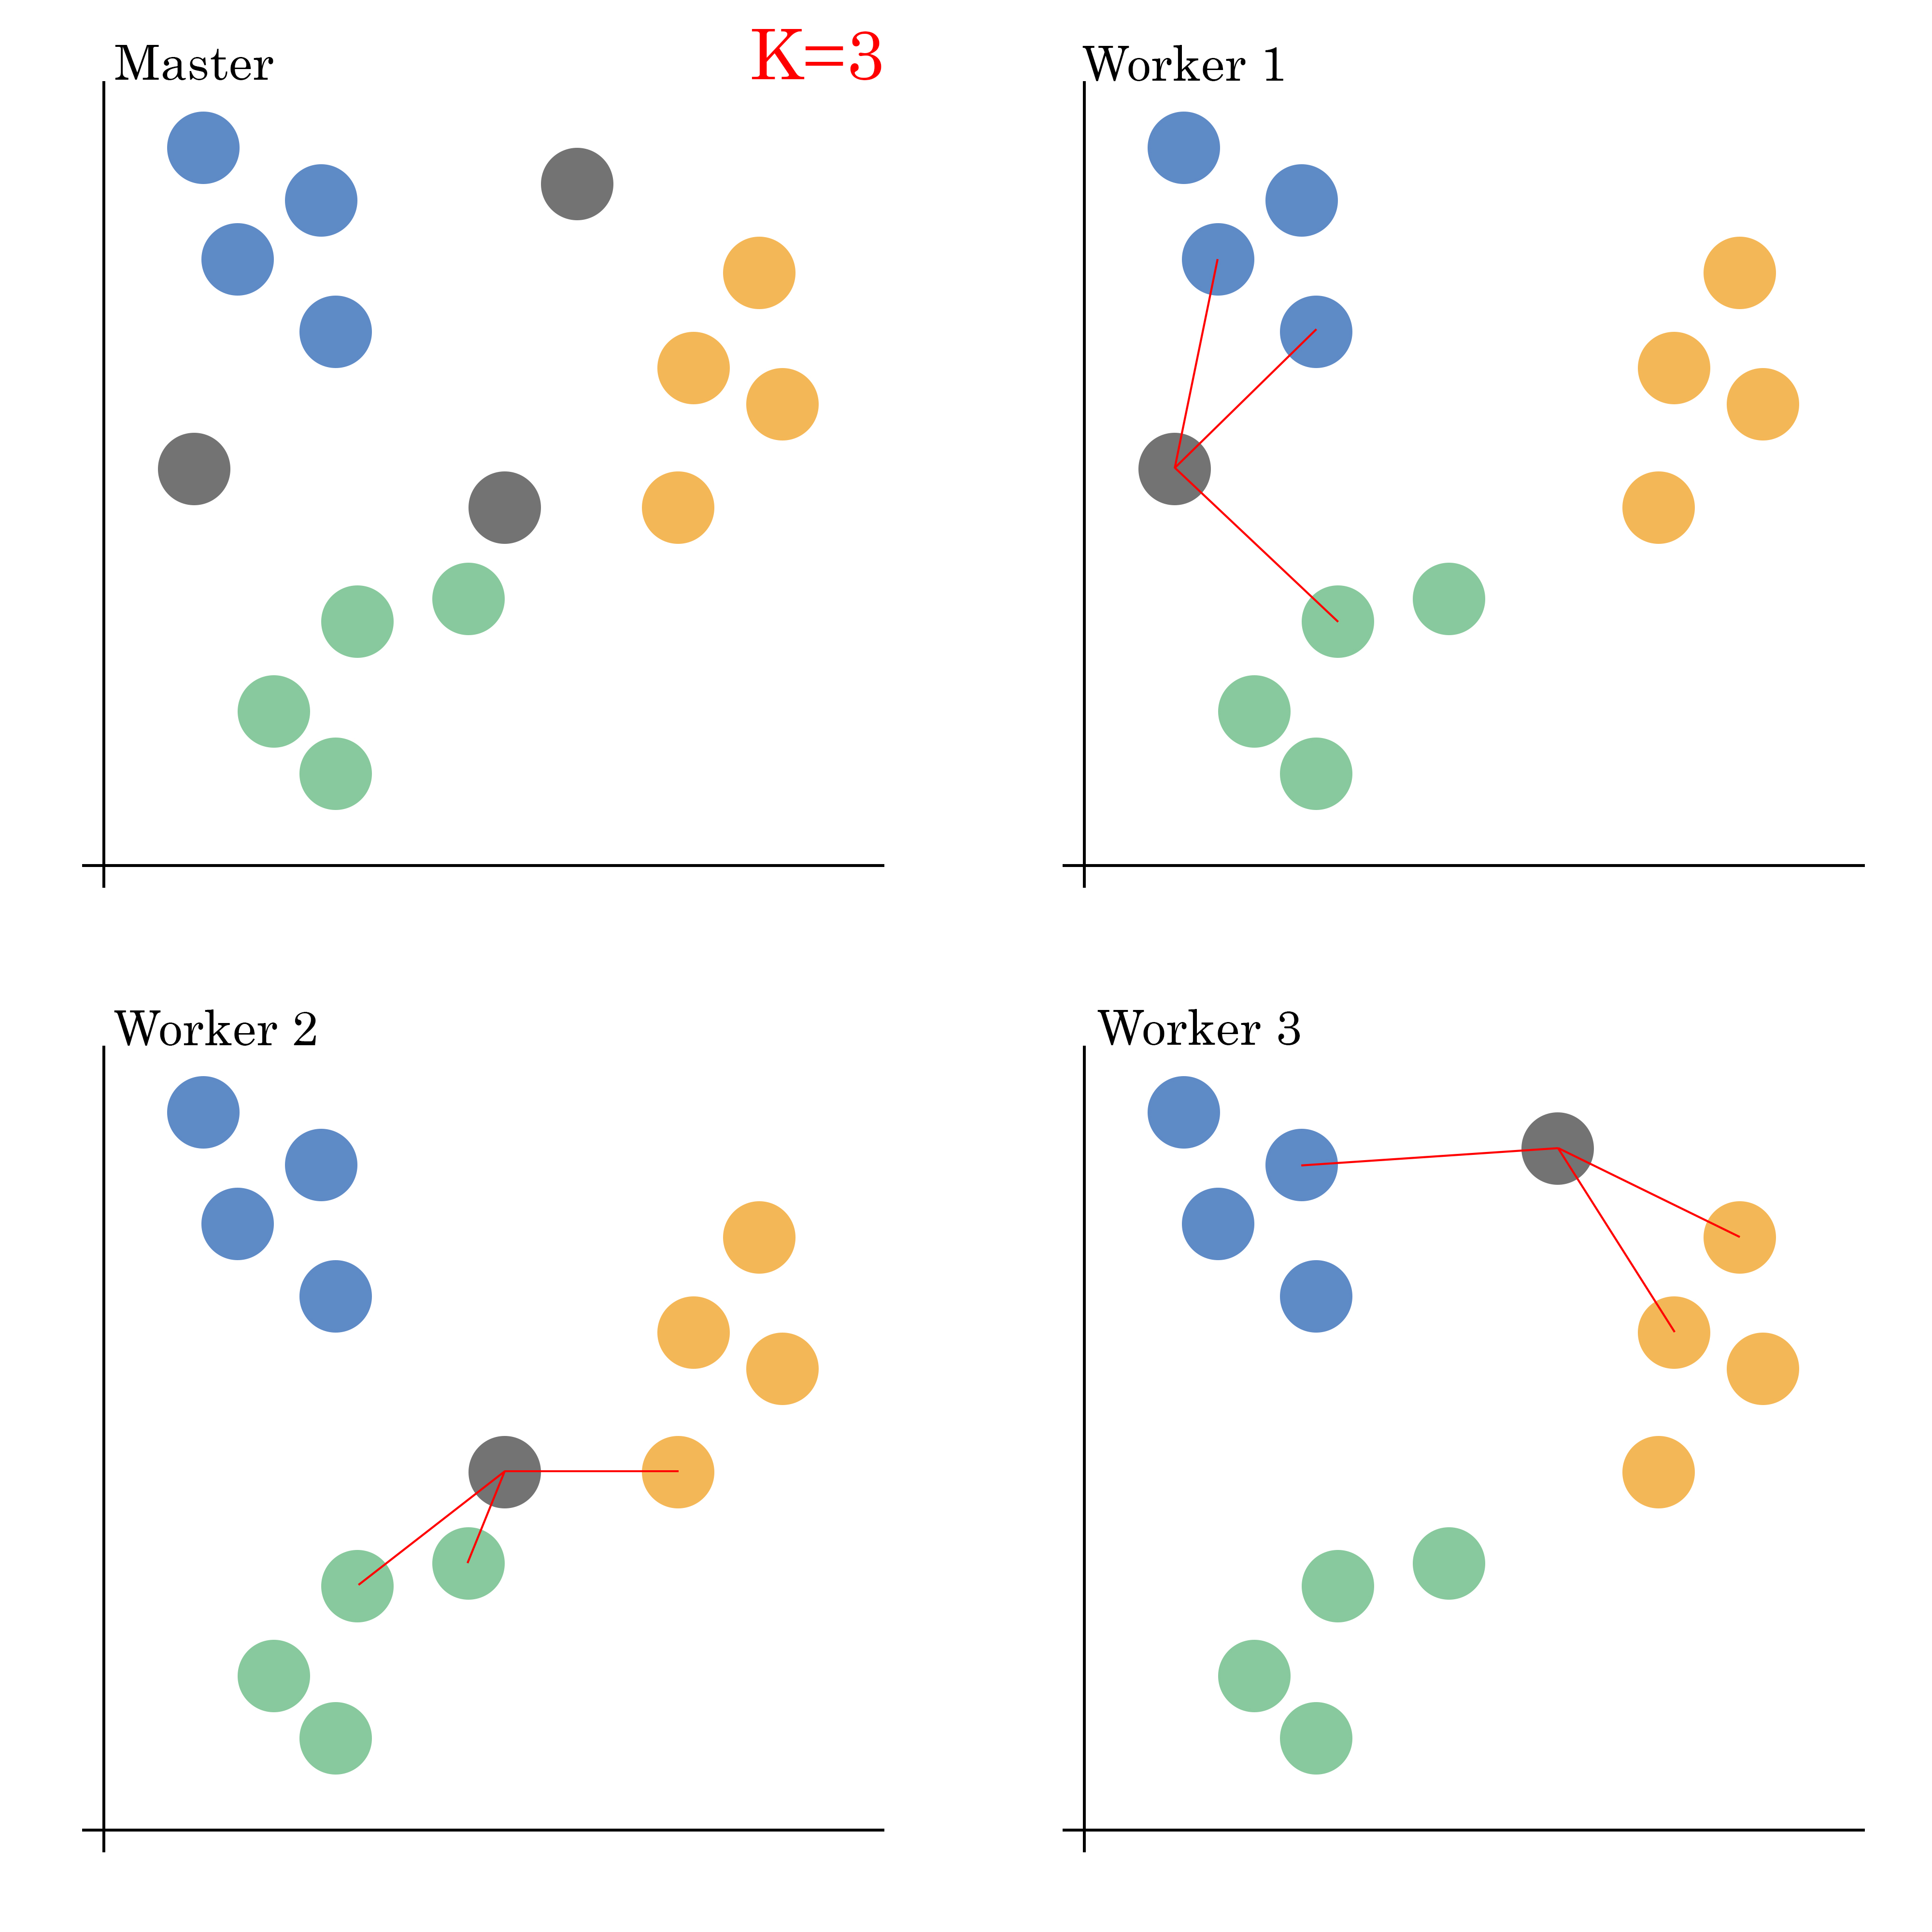
\includegraphics[width=\textwidth]{images/chapter_3/knn_mpi2}
				\caption{Segunda}
				\label{fig:knn2}
			\end{subfigure}
			
			\caption{MPI - KNN impplemetaciones}
			\label{fig:knnmpi}
		\end{figure}

		El proceso Master (el de la esquina superior izquierda) tiene el dataset completo. En la primera implementación (gráfico de la izquierda) divide la población categorizada entre los procesos. Y la segunda implementación (gráfico de la derecha) tiene una copia entera de la población categorizada en todos los procesos.
		
		
		Para realizar una búsqueda del mejor valor para K, al contrario que en K-Medias, no hace falta repetir varias veces el mismo algoritmo, el proceso es determinista. Es decir, con la misma población, siempre sale la misma predicción. A no ser que se cambie el orden de predicción y se actualice la población a predecir. No es necesario ejecutar varias veces el mismo algoritmo, pero sí puede ser útil variar el número de vecinos (K). Las mejoras de esta búsqueda son las mismas que en el algoritmo anterior. Aplicar la mejora MPI e iterar cambiando los valores de K, o ejecutar de manera secuencial en varios procesos.

\newpage

\section{Aprendizaje por refuerzo}

	Los algoritmos de este aprendizaje actualizan iterativamente las estimaciones de calidad de las acciones permitidas en el entorno de desarrollo. 
	
	\subsection{Q-Learning}
		Dichas estimaciones se almacenan en una Q-Table, representada como una matriz en la que cada fila es un estado, y las columnas son las acciones disponibles. 
		
		Para este algoritmo nos centramos en la técnica de \textbf{minimizar las acciones}. El agente se encuentra en un laberinto, el tamaño y la semilla es variable por parámetros de inicialización. Tiene que recorrer el laberinto desde un punto inicial hasta una celda destino, en el menor número de acciones posibles. Las acciones disponibles para el agente son solo de movimiento: arriba, derecha, abajo e izquierda. No puede atravesar ni situarse en un muro del laberinto. Hay que fijar unas recompensas con las acciones tomadas. 	
		\begin{itemize}
			\item Si se choca con un muro castigamos al agente con valores altos para que no haga esas acciones.
			\vspace*{-0.2cm}
			\item Al moverse, el agente recibe un castigo pequeño para que aprenda a minimizar las operaciones.
			\vspace*{-0.2cm}
			\item Al llegar a la meta le damos una recompensa alta. 		
			\vspace*{-0.2cm}
		\end{itemize}
	
		Con estas recompensas aprende a llegar a la meta minimizando las acciones ejecutadas. El código que genera los laberintos ha sido implementado por @ChlouisPy en github\cite{MazeGenerator}

	
		\subsubsection{Preprocesado}
		
			Modificando la Q-Table, convertiendola en un array bidimensional, en el cual no se almacenen las acciones que no deseamos que realice el agente, como puede ser chocarse con un muro, puede reducir el tiempo de cómputo, al no perder tiempo chocando con paredes. Además de reducir la complejidad espacial al eliminar los estados inaccesibles, reduciendo el número de estados, pero añadiendo un nuevo array bidimensional de acciones para cada estado. 
			
			Este preprocesado tiene complejidad cuadrática \textit{O(4*N2) $\equiv$ O(N2)}. Recorre toda la matriz, compruebando para cada celda si no es un muro, y en caso afirmativo comprueba las cuatro acciones permitidas y almacena las disponibles en los arrays bidimensionales de valores-Q y acciones. Con tamaños de laberintos pequeños no hace falta paralelizar el preprocesado, porque no se consigue reducir el tiempo significativamente.
			
		\subsubsection{Búsqueda de hiper-parámetros ideales}
		
			Los hiper parámetros ($\alpha$, $\gamma$, $\epsilon$) son muy importantes para el desarrollo del agente en el entorno. Una mala configuración de estos hace que sobre aprenda o no aprenda correctamente, generando bucles infinitos. Por este motivo es importante comprobar las diferentes combinaciones de hiper parámetros, y ver cuales funcionan correctamente en el entorno. La búsqueda en laberintos grandes es muy lenta. Hay que comprobar muchas combinaciones entre los hiper parámetros y los episodios del entrenamiento. Por eso es más útil desarrollar el algoritmo Deep Q-Learning que no tiene problemas con los estados, al usar una red neuronal. Pero si queremos usar el algoritmo básico de Q-Learning, hay que realizar una búsqueda exhaustiva en el entorno ejecutando muchas  combinaciones de hiper parámetros.
	
			Con MPI se puede procesar ejecutando de manera secuencial en diferentes procesos. Idea mencionada en otros algoritmos. El master envía configuraciones diferentes a los workers. Si aplicamos una precisión de 0.1, y reduciendo el número de mensajes, cada worker ejecuta 9 veces el algoritmo, aumentando un 10\% en cada iteración el hiper parámetro $\epsilon$ (el que controla la toma de decisiones). 
			
			%\newpage
			
			\begin{figure}			
			\begin{mdframed}[roundcorner=5pt]
				El master envía configuraciones diferentes a los workers. Si aplicamos una precisión de 0.1, y reduciendo el número de mensajes, cada worker ejecuta 9 veces el algoritmo, aumentando un 10\% en cada iteración el hiper parámetro $\epsilon$ (el que controla la toma de decisiones). Al terminar una ejecución el worker escribe en un fichero de texto: 
				
				
				\begin{tcolorbox}[boxrule=0.5pt, fontupper=\small]			
					- La id del proceso. \\
					- Los hiper parámetros ejecutados.v
					- El tiempo de ejecución \\
					- Como termina:\\
					$\rightarrow$ Bucle en entrenamiento.\\
					$\rightarrow$ Bucle en evaluación.\\
					$\rightarrow$ Movimientos. Si termina correctamente.
						
					
				\end{tcolorbox}
				
			\end{mdframed}
			\caption{RL - Búsqueda de hiperparámetros}
			\label{fig:rl_busqueda}
			\end{figure}
			
			Los bucles se detectan de diferentes formas. En el entrenamiento, si un episodio tarda más de x segundos, es porque está en un bucle y estos hiper parámetros no funcionan. En la evaluación se comprueba llevando una cuenta de los últimos 4 estados visitados. 
			\begin{center}
				\textit{Estados[0]==Estados[2] and Estados[1]==Estados[3] and Estados[0]!=Estados[1]: }
			\end{center}
	
	
	
			\begin{flushleft}
				Las posibles mejoras de este algoritmo son más complejas, se puede:		
			\end{flushleft}
			\vspace{-0.9cm}
			\begin{enumerate}
				\item Dividir el entorno entre los procesos.
				\vspace*{-0.2cm}
				\item Ejecutar el algoritmo en los workers y juntar las experiencias.				
			\end{enumerate}
	
		\subsubsection{Dividir el entorno}
			Al dividir el laberinto entre los procesos, cada proceso controla una zona, y se genera un flujo constante de episodios. Cuando un agente sale del dominio de un proceso, este le manda un mensaje al proceso que controla esa parte del laberinto, con la posición en la que entra. Figura \ref{fig:rlmpi}. El master se encarga de iniciar a los agentes y cuando sale de su dominio genera otro agente. Para garantizar que funcione el master no puede recibir agentes de los workers, en caso contrarior no se podría garantizar el flujo de nuevos episodios. Pero solo puede exister \textit{M} agentes en todos los procesos (siendo \textit{M} el número de procesos ejecutados), debido a que un proceso solo puede gestionar a lo sumo un agente. Como cada proceso tiene su propio dominio, la Q-Table se divide entre estos. Aplicando la mejora con el preprocesado, es la misma idea pero con los dos arrays bidimensionales (acciones y Q-valores). 
			
			Hay que tener en cuenta los límites de cada proceso, para cuando el agente salga fuera de estos, envíe un mensaje con la posición en la que entra al proceso correcto. Es un flujo constante de agentes nuevos, por eso es mejor que una vez salga del primer proceso (el que genera los agentes), no pueda volver a entrar, asi simplificando la lógica de programación.
			
			\begin{figure}[!h]
				\centering
				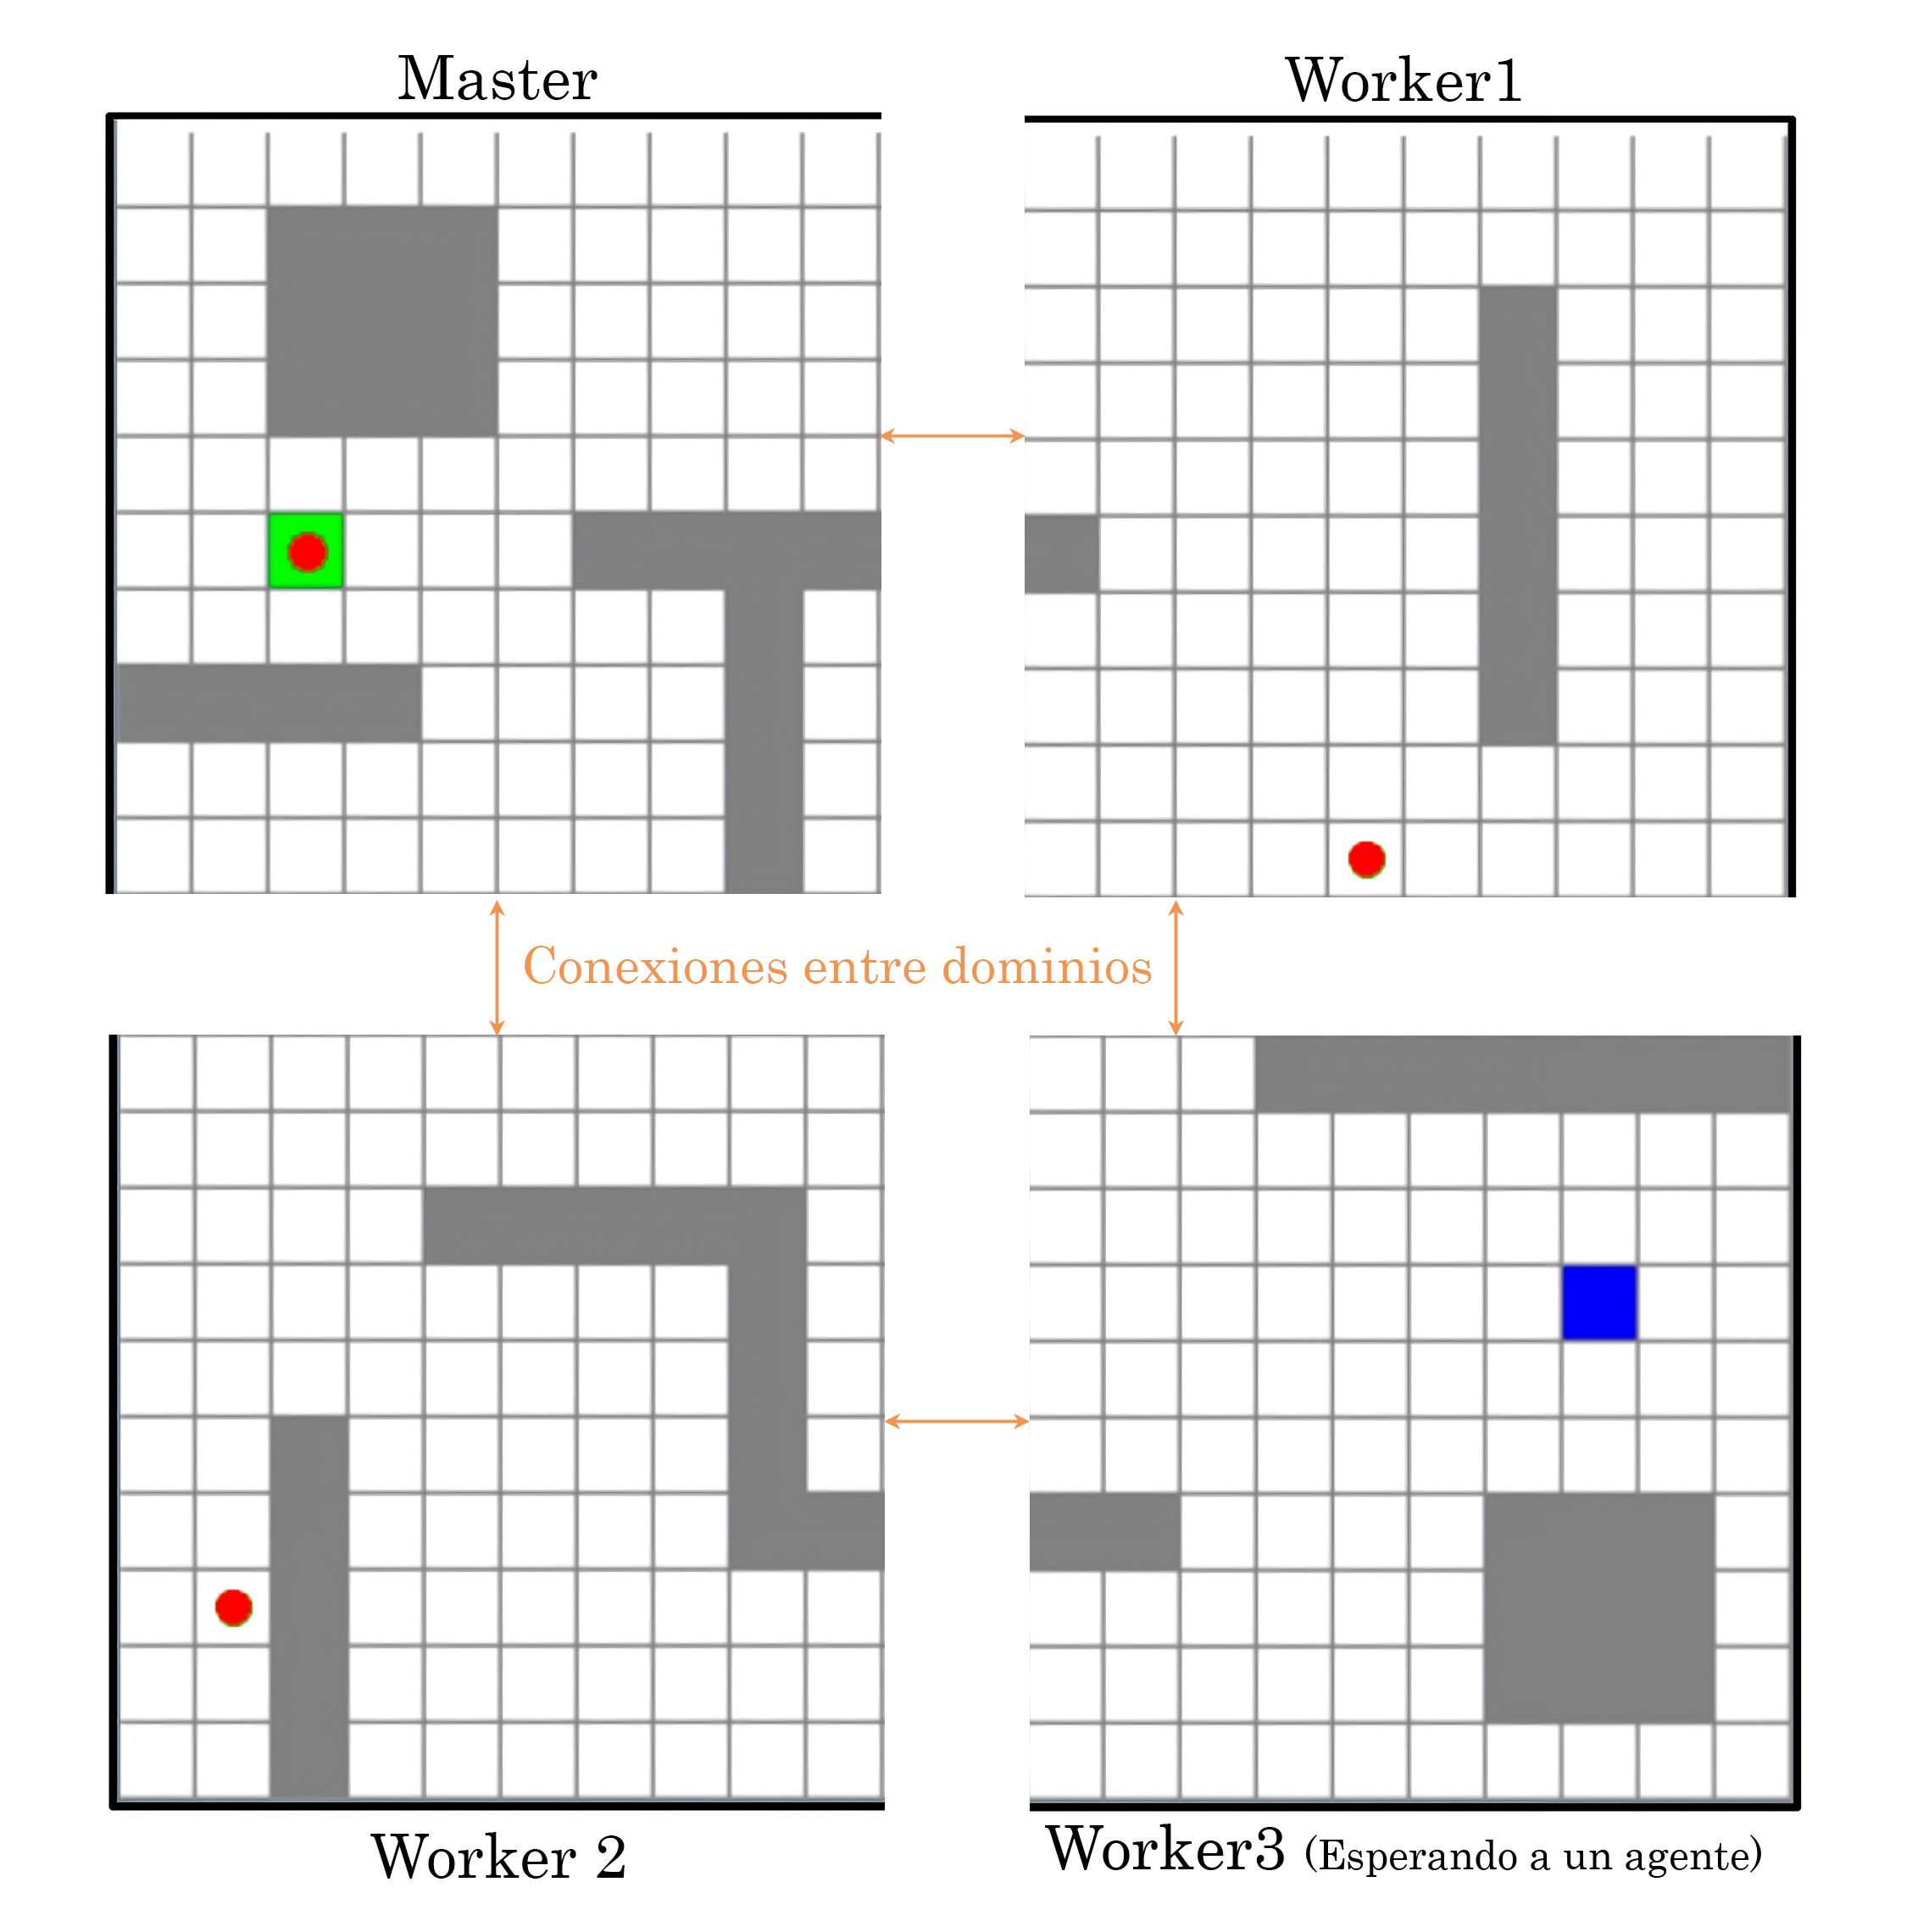
\includegraphics[width=0.65\textwidth]{images/chapter_3/rl_mpi}	
				\caption{RL - División del entorno}
				\label{fig:rlmpi}
			\end{figure}
	
		\subsubsection{Juntar experiencias}
	
			Ejecutar en varios procesos el algoritmo, funciona. El master recolecta las experiencias de los workers, haciendo la media de los valor-Q obtenidos de los procesos, así calculando la mejores acciones para cada estado. 
			
			Es mucho mejor inicializar el algoritmo desde distintos puntos, para así explorar todo el laberinto y encontrar el mejor camino en menos tiempo. Al menos un worker inicia desde el punto de inicio que se desea evaluar, pues de lo contrario no se podría garantizar que visiten la zona del inicio, y obtengan las estimaciones correctas para llegar al destino.
			
			
	
	
	
	
	\subsection{DQN}
	
		Este algoritmo utiliza redes neuronales para obtener la mejor acción para un determinado estado, así eliminando los problemas que tiene el algoritmo anterior. Con es método podemos abarcar entornos más complejos, y por eso se propone el juego de atari Pac-Man, centrándonos en obtener el mayor número de monedas antes de provocar una condición de finalización. Antes de profundizar en el algoritmo de IA, explicamos el entorno del problema a resolver:
		\vspace{-0.5cm}
		\begin{itemize}		
			\item Acciones disponibles. Como en el algoritmo anterior, son de movimiento. El agente y los fantasmas no pueden atravesar muros.
			\vspace*{-0.2cm}
			\item Entorno. Laberinto con muros, del cual no se puede escapar.
			\item Objetos del juego. 
			\vspace*{-0.3cm}
				\subitem Pac-Man, el agente que mueve el usuario. Su objetivo es comer todos los puntos.
				\vspace*{-0.3cm}
				\subitem Fantasmas, se mueven siguiendo unos objetivos en el laberinto.
				\vspace*{-0.3cm}
				\subitem Túneles. Puntos que se conectan de manera toroidal para no salir del
				\vspace*{-0.3cm}
				\subitem Puntos (pellets en ingles). Son las "monedas" que el agente tiene que recoger.
				\vspace*{-0.3cm}
				\subitem Puntos de energia (powers). Si el agente consume uno, durante un periodo de tiempo es invencible y puede comer a los fantasmas.
				
				 laberinto.				
			\vspace*{-0.3cm}
			\item Condiciones de finalización. Ganar obteniendo todas las monedas del laberinto o perder si un fantasma come al agente. 			
		\end{itemize}
		
		\begin{flushleft}
			Los fantasmas tienen una IA interesante, pues tienen sus propios estados y cada uno tiene unos puntos objetivos que siguen para intentar comer al agente. Los estados son los siguientes:
		\end{flushleft}
		\vspace{-0.9cm}
		\begin{itemize}
			\item Chase. Cada fantasma sigue unos puntos en movimiento.
			\vspace*{-0.3cm}
			\item Scatter. Sigue un punto estático fuera del laberinto para dar vueltas en una determinada zona.
			\vspace*{-0.3cm}
			\item Frightened. El agente puede comerlos, se mueve de manera aleatoria al llegar a una intersección.
			\vspace*{-0.3cm}
			\item Eaten. Han sido comidos y se encuentran en su casa esperando a salir. (Implementado de forma que espera 3 movimientos del agente para salir)
		\end{itemize} 
		
		\begin{flushleft}
			En la estado \textit{Chase} los fantasmas se mueven de la siguiente forma:
		\end{flushleft}
		
		\vspace{-0.9cm}
		\begin{itemize}
			\item Blinky (Rojo): Persigue directamente al agente.
			\vspace*{-0.3cm}
			\item Pinky (Rosa): Persigue la celda cuatro posiciones adelantada a donde apunta el agente. Si el agente mira hacia arriba, también añade cuatro celdas hacia la izquierda
			\vspace*{-0.3cm}
			\item Inky (Azul): Persigue una celda en concreto que se calcula de la siguiente forma. Primero se calcula una posición como lo hace el fantasma rosa pero en vez de cuatro celdas, se hace con dos. El objetivo se calcula al añadir el vector de distancia de la posición del fantasma rojo a esta posición.
			\vspace*{-0.3cm}
			\item Clyde (Naranja): Si está a ocho o más celdas de distancia del agente, lo persigue. En caso contrario sigue su objetivo del estado Scatter.
		\end{itemize}
		
		El laberinto y el juego han sido creados desde cero para facilitar el aprendizaje del la IA, con estados mas sencillos y poder hacer los cambios necesarios en un futuro. El laberinto se almacena en un fichero de texto, para representar las celdas vacias, muros, puntos o puntos de poder con números enteros (0, 1, 2 y 3 respectivamente).
		
		
		
		
		\subsubsection{Entrenamiento}
			
			La fase de entrenamiento es crucial, pues modifican los valores de la red neuronal para que tome las mejores decisiones en cada estado, haciendo que el agente pueda terminar el problema sin perder.	El entrenamiento se puede realizar de varias formas.	
			
							
			Si mantenemos el mismo estado inicial, el agente empieza siempre en el mismo punto, y depende mucho de los hiperparámetros, además de la aleatoriedad. El agente empieza a investigar el entorno de manera aleatoria, y es muy probable que los fantasmas alcancen al agente bastante rápido sin explorar mucho el entorno. Por eso es mejor añadir varios estados iniciales para que pueda investigar el entorno de manera más eficiente. Hay que tener en cuenta que los estados iniciales tienen que ser puntos accesibles desde el estado inicial original. El agente no puede saltar a otros puntos sin coger los puntos del laberinto (Figura \ref{fig:pacman_states}), si entrenamos con puntos aleatorios sin cambiar el estado del laberinto, al ejecutar el algoritmo con los mejores valores obtenidos, no habrá servido de nada, pues son estados que el agente no va a alcanzar nunca.
			
		
			\begin{figure}[!h]
				\centering
				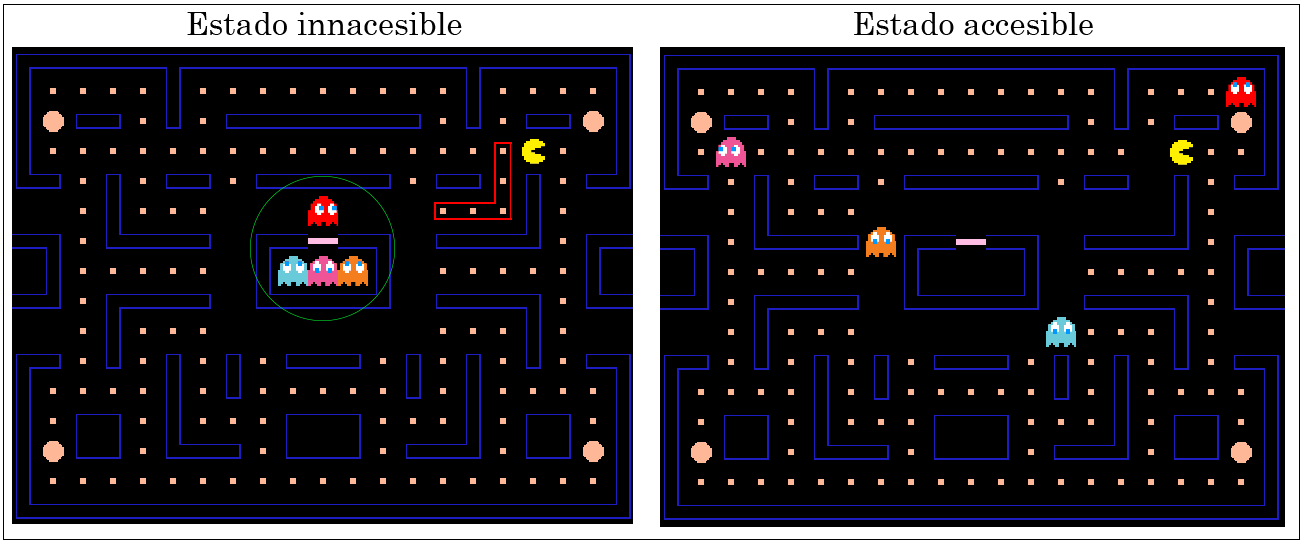
\includegraphics[width=1\textwidth]{images/chapter_3/pacman_states}	
				\caption{DQN - Estados del entorno}
				\label{fig:pacman_states}
			\end{figure}
			
			En la ejecución de la izquierda, el agente empieza en una posición aleatoria, sin cambiar los objetos del entorno. Este estado nunca se va a ejecutar, pues necesita coger los puntos del camino y cambiar las posiciones de los fantasmas, como se puede ver en la ejecución de la derecha.
			
		\subsubsection{Mejoras MPI}
		
			Al usar redes neuronales, se pueden aplicar las mejoras que se van a comentar en la sección de redes neuronales \ref{sec:redes_neu}. No se pueden aplicar las mejoras del algoritmo anterior, pues no es una matriz que se pueda dividir el trabajo, es una red neuronal cuyos pesos varían al ejecutar acciones en estados.
		
			
		
		
		
			
		
		
	
		
	
	\newpage
	


\section{Algoritmos Evolutivos}
	Los algoritmos evolutivos son sencillos de paralelizar, debido a que son procesos que se repiten muchas veces, y se ejecutan en muchos individuos.
	
	\begin{enumerate}
		\item \textbf{Inicialización.} Dados los parámetros iniciales se crea la población, con los individuos deseados. Hay diferentes tipos, con sus respectivas características.
		\begin{itemize}
			\item Binarios. Estos individuos son fáciles de inicializar, pero ralentizan la comunicación entre procesos, debido a tener que enviar muchos bits.
			\item Reales. Parecidos a los binarios pero estos son más portables.
			\item Árboles. Más lentos para inicializar y difíciles de tratar.
		\end{itemize}
		
		\item \textbf{Evaluación.} Este es el método que más tiempo de ejecución puede llegar a consumir. Varía dependiendo del tipo de individuo del problema.
		
		\item \textbf{Selección.} Se seleccionan a los individuos. El tiempo depende de los métodos de selección aplicados, pero suelen ser lineales.
		
		\item \textbf{Cruce.} Con una cierta probabilidad, se cruzan 2 individuos del conjunto seleccionado. Tienen un mayor coste que selección.
		
		\item \textbf{Mutación.} Igual que el cruce tiene una probabilidad para mutar. Parecido a cruce, pero un poco más rápido.
	\end{enumerate}
	
	Para cada tipo de individuos se desarrollan unos problemas.\\
	1. Binario, con un intervalo dado y una precisión, queremos calcular el valor máximo o mínimo para ciertas funciones. Los valores fitness se calculan con la representación real del cromosoma, que varía dependiendo de la precisión que se le asigna al ejecutar el algoritmo. Por lo que hay que convertir de binario a real.
	Este problema se ejecuta bastante rápido. Reducir su tiempo de ejecución es desafiante.\\
	2. Real. Aeropuertos con un número variable de vuelos y pistas. Queremos calcular el sumatorio de tiempos mínimos de retraso para que los aviones aterricen en el aeropuerto. Cada avión tiene asignada la hora de aterrizaje para cada pista, y hay un tiempo mínimo de separación entre vuelos que aterrizan en cada pista. Se puede resolver con vuelta atrás pero tiene un coste exponencial (inviable). El valor fitness tiene coste \textit{O(NumAviones*NumPistas) $\equiv$ O(\(N^{2}\))}. Se calcula:
	
	\lstset{language=python, 
		breaklines=true, 
		basicstyle=\footnotesize,
		backgroundcolor=\color{lightergray},
		commentstyle=\color{green_comment},}
	\begin{lstlisting}
 fitness=0
 for avion in aviones:
 for pista in range(pistas): # Calculamos TLA para cada pista
 TLA = maximo(TLA(vuelo_anterior) + SEP[vuelo_anterior][vuelo_actual], TEL)
 # Se asigna el vuelo actual a la pista con minimo TLA calculado
 fitness+=(menor_TLA-menor_TEL)^2
 # menor_TEL: menor TEL de ese vuelo con todas las pistas		
	\end{lstlisting}
	
	\noindent El tiempo de ejecución para este problema depende de la función de evaluación, que varía dependiendo del número de aviones y pistas. 
	
	3. Árbol, tenemos una matriz de enteros que representa un jardín. 1: césped y                 0: césped podado. Queremos maximizar el área podada. Para ello el agente tiene unas acciones que puede ejecutar.
	El coste temporal de este algoritmo viene dado principalmente por la función de evaluación. Ejecuta la simulación en la matriz hasta cumplir un determinado número de ticks (acciones realizadas), que es proporcional al número de filas y columnas de la matriz. Aunque las funciones de cruce y mutación también tardan en ejecutarse, debido al control de punteros.
	
	
	
	\begin{flushleft}
		Cada una de las siguientes mejoras MPI se pueden configurar para cada tipo de individuo.\\
		1. Dividir la población en subpoblaciones.\\
		2. Modelo de islas.\\
		3. PipeLine. (Figura \ref{fig:pevpipe})\\
	\end{flushleft}
	
	La primera implementación, de dividir la poblacion entre procesos, se puede paralelizar fácilmente. El master recibe de los Workers las subpoblaciones inicializadas y evaluadas, y comienza el bucle principal del algoritmo, en el cual:
	\begin{itemize}
		\item El master se encarga de hacer la selección, y enviarla dividida a los workers. Mientras los workers trabajan, el master almacena el progreso de los mejores individuos de cada generación.
		\item Los workers reciben la selección, la cruzan, mutan y evalúan. Al finalizar estos procesos mandan la subpoblación al master para empezar la siguiente iteración.
	\end{itemize}
	
	Para el \textbf{modelo de islas}, se aplica la idea de mejoras pasadas, en cada proceso se ejecuta el algoritmo. Todos tienen el mismo tamaño, pero distintas poblaciones. Hay varios tipos de comunicaciones en esta mejora. Cada cierto tiempo se reinicia la población con los mejores individuos generales (de todos los procesos).

	\begin{itemize}
		\item Estrella. Solo hay comunicaciones master-worker. El master recibe los mejores individuos.
		\item En red. No hay proceso master, todos los procesos ejecutan el algoritmo. Todos los procesos están en comunicación constante, mandando los mejores individuos para el reinicio de la población.
		\item En anillo. Tampoco hay proceso master, los procesos se comunican como una lista enlazada.
	\end{itemize}
	
	Segmentar el algoritmo entre los procesos, provoca un flujo constante de generaciones. Cada proceso se encarga de un método. El master se encarga de generar cuatro poblaciones distintas y las evalúa para mandarlas al worker que se encarga de la selección. El master no genera más poblaciones, y pasa a un estado de recepción mejores individuos. Las poblaciones van evolucionando conforme avanzan por el pipeline. El último worker se encarga de la evaluación, que envía al worker de selección, y al master.
	
	\begin{figure}[!h]
		\centering
		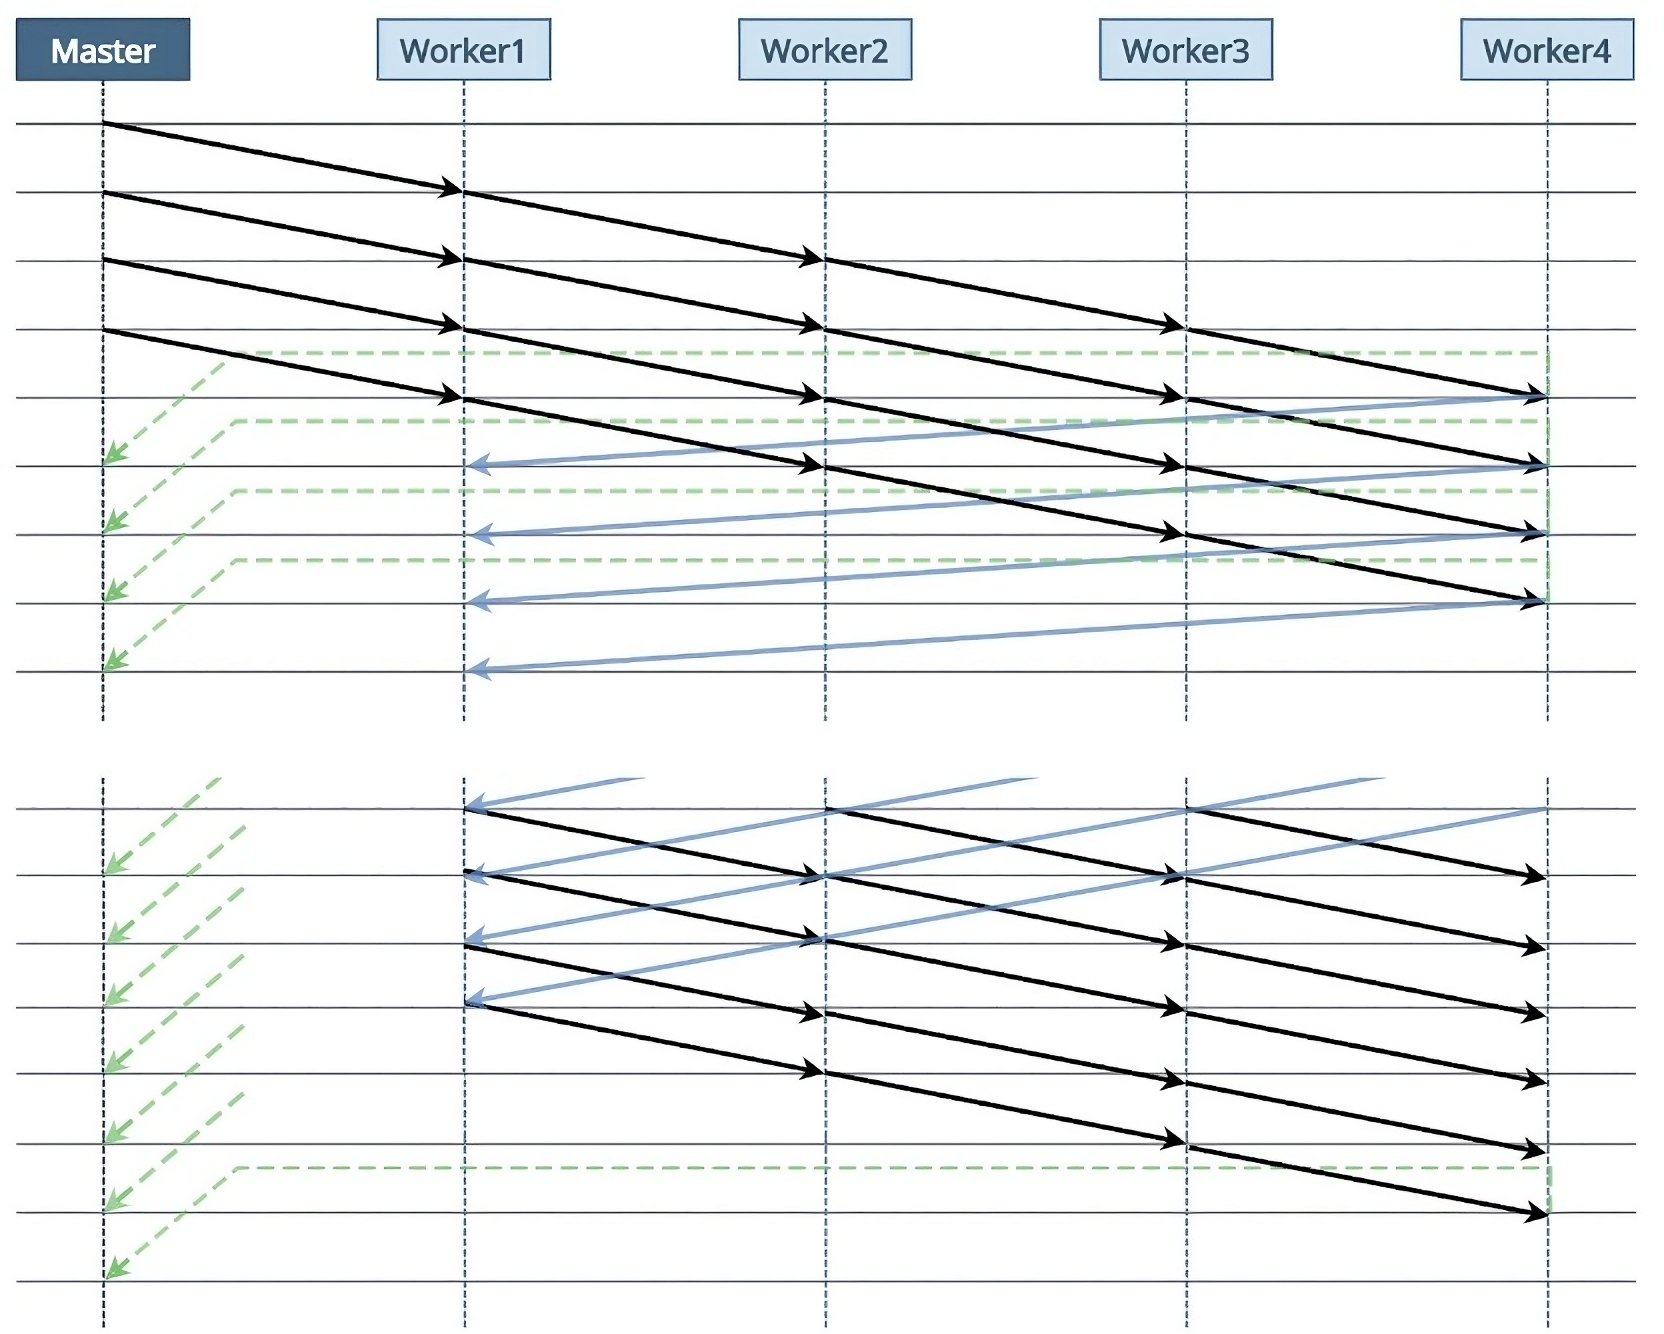
\includegraphics[width=0.65\textwidth]{images/chapter_3/pev_mpi3}
		\caption{MPI - PEV PipeLine}
		\label{fig:pevpipe}
	\end{figure}

	Se puede reducir el tiempo de ejecución si comprobamos que métodos tardan más, añadiendo más procesos para reducir la carga de trabajo.
	
	
	
	
	


\section{Redes Neuronales}
\label{sec:redes_neu}	
	Esta poderosa herramienta de aprendizaje supervisado, está diseñada para reconocer patrones complejos y realizar diversas tareas. Aprende con un proceso iterativo de entrenamiento, ajustando las conexiones entre neuronas. Este proceso secuencial es complejo de paralelizar. Al finalizar una predicción el modelo se tiene que actualizar propagando hacia atrás.
	
	Nos centramos en la técnica de \textbf{predicción}. La capa de entrada está formada por dos neuronas, cada individuo son variables numéricas que representan, la altura y el peso de una persona, y aprende a predecir el Índice de Masa Corporal (IMC). La capa de entrada y salida no varían, pero la capa oculta se puede modificar libremente, aumentando el tiempo en la fase de entrenamiento.
	
	
	Como en algoritmos pasados, necesitamos encontrar la mejor tasa de aprendizaje, para que aprenda lo mejor posible. Por lo que diseñamos una programa MPI, en el cual se ejecutan en varios procesos el mismo algoritmo con diferentes tasas de aprendizaje y repeticiones para el entrenamiento. El speedup es proporcional al número de procesos.
	
	\begin{flushleft}
		Como en el algoritmo anterior, se puede aplicar un pipeline para que haya un flujo de mensajes, pero esta vez en vez de ser unidireccional es bidireccional, al tener que actualizar los pesos de las neuronas al predecir un individuo.\\	
		1. PipeLine\\
		2. Dividir el trabajo en procesos
	\end{flushleft}
	
	Segmentar el proceso de entrenamiento puede llegar a ser beneficioso. Cada proceso se encarga de una capa de la red neuronal, siendo el master el encargado de enviar individuos de la población categorizada. El último worker controla la capa de salida, con las etiquetas calcula el error y lo propaga hacia atrás. Para el correcto funcionamiento, hay que crear un buen diseño para tener un flujo constante de mensajes. Figura \ref{fig:redneumpipipe}.
	
	
	
	\begin{enumerate}
		\item El master envía un número proporcional de individuos al número de procesos ejecutándose. Luego entra en un bucle en el cual recibe el error, actualiza, y envía otro individuo. Para finalizar recibe el mismo número de individuos que envió al principio y actualiza.
		\item El último worker solo recibe las predicciones y calcula el error.
		\item Los workers de la capa oculta tienen un proceso más complejo. Primero reciben un número de individuos proporcional a su id, los procesan y envían. Después entran en un bucle en el cual:			
		\begin{itemize}
			\item Reciben, de la capa siguiente, los errores, actualizan sus pesos y envían a la capa anterior.			
			\item Reciben, de la capa anterior, los nuevos individuos, procesan y propagan hacia adelante.
		\end{itemize}		
		
	\end{enumerate}
	
	\begin{figure}[!h]
		\centering
		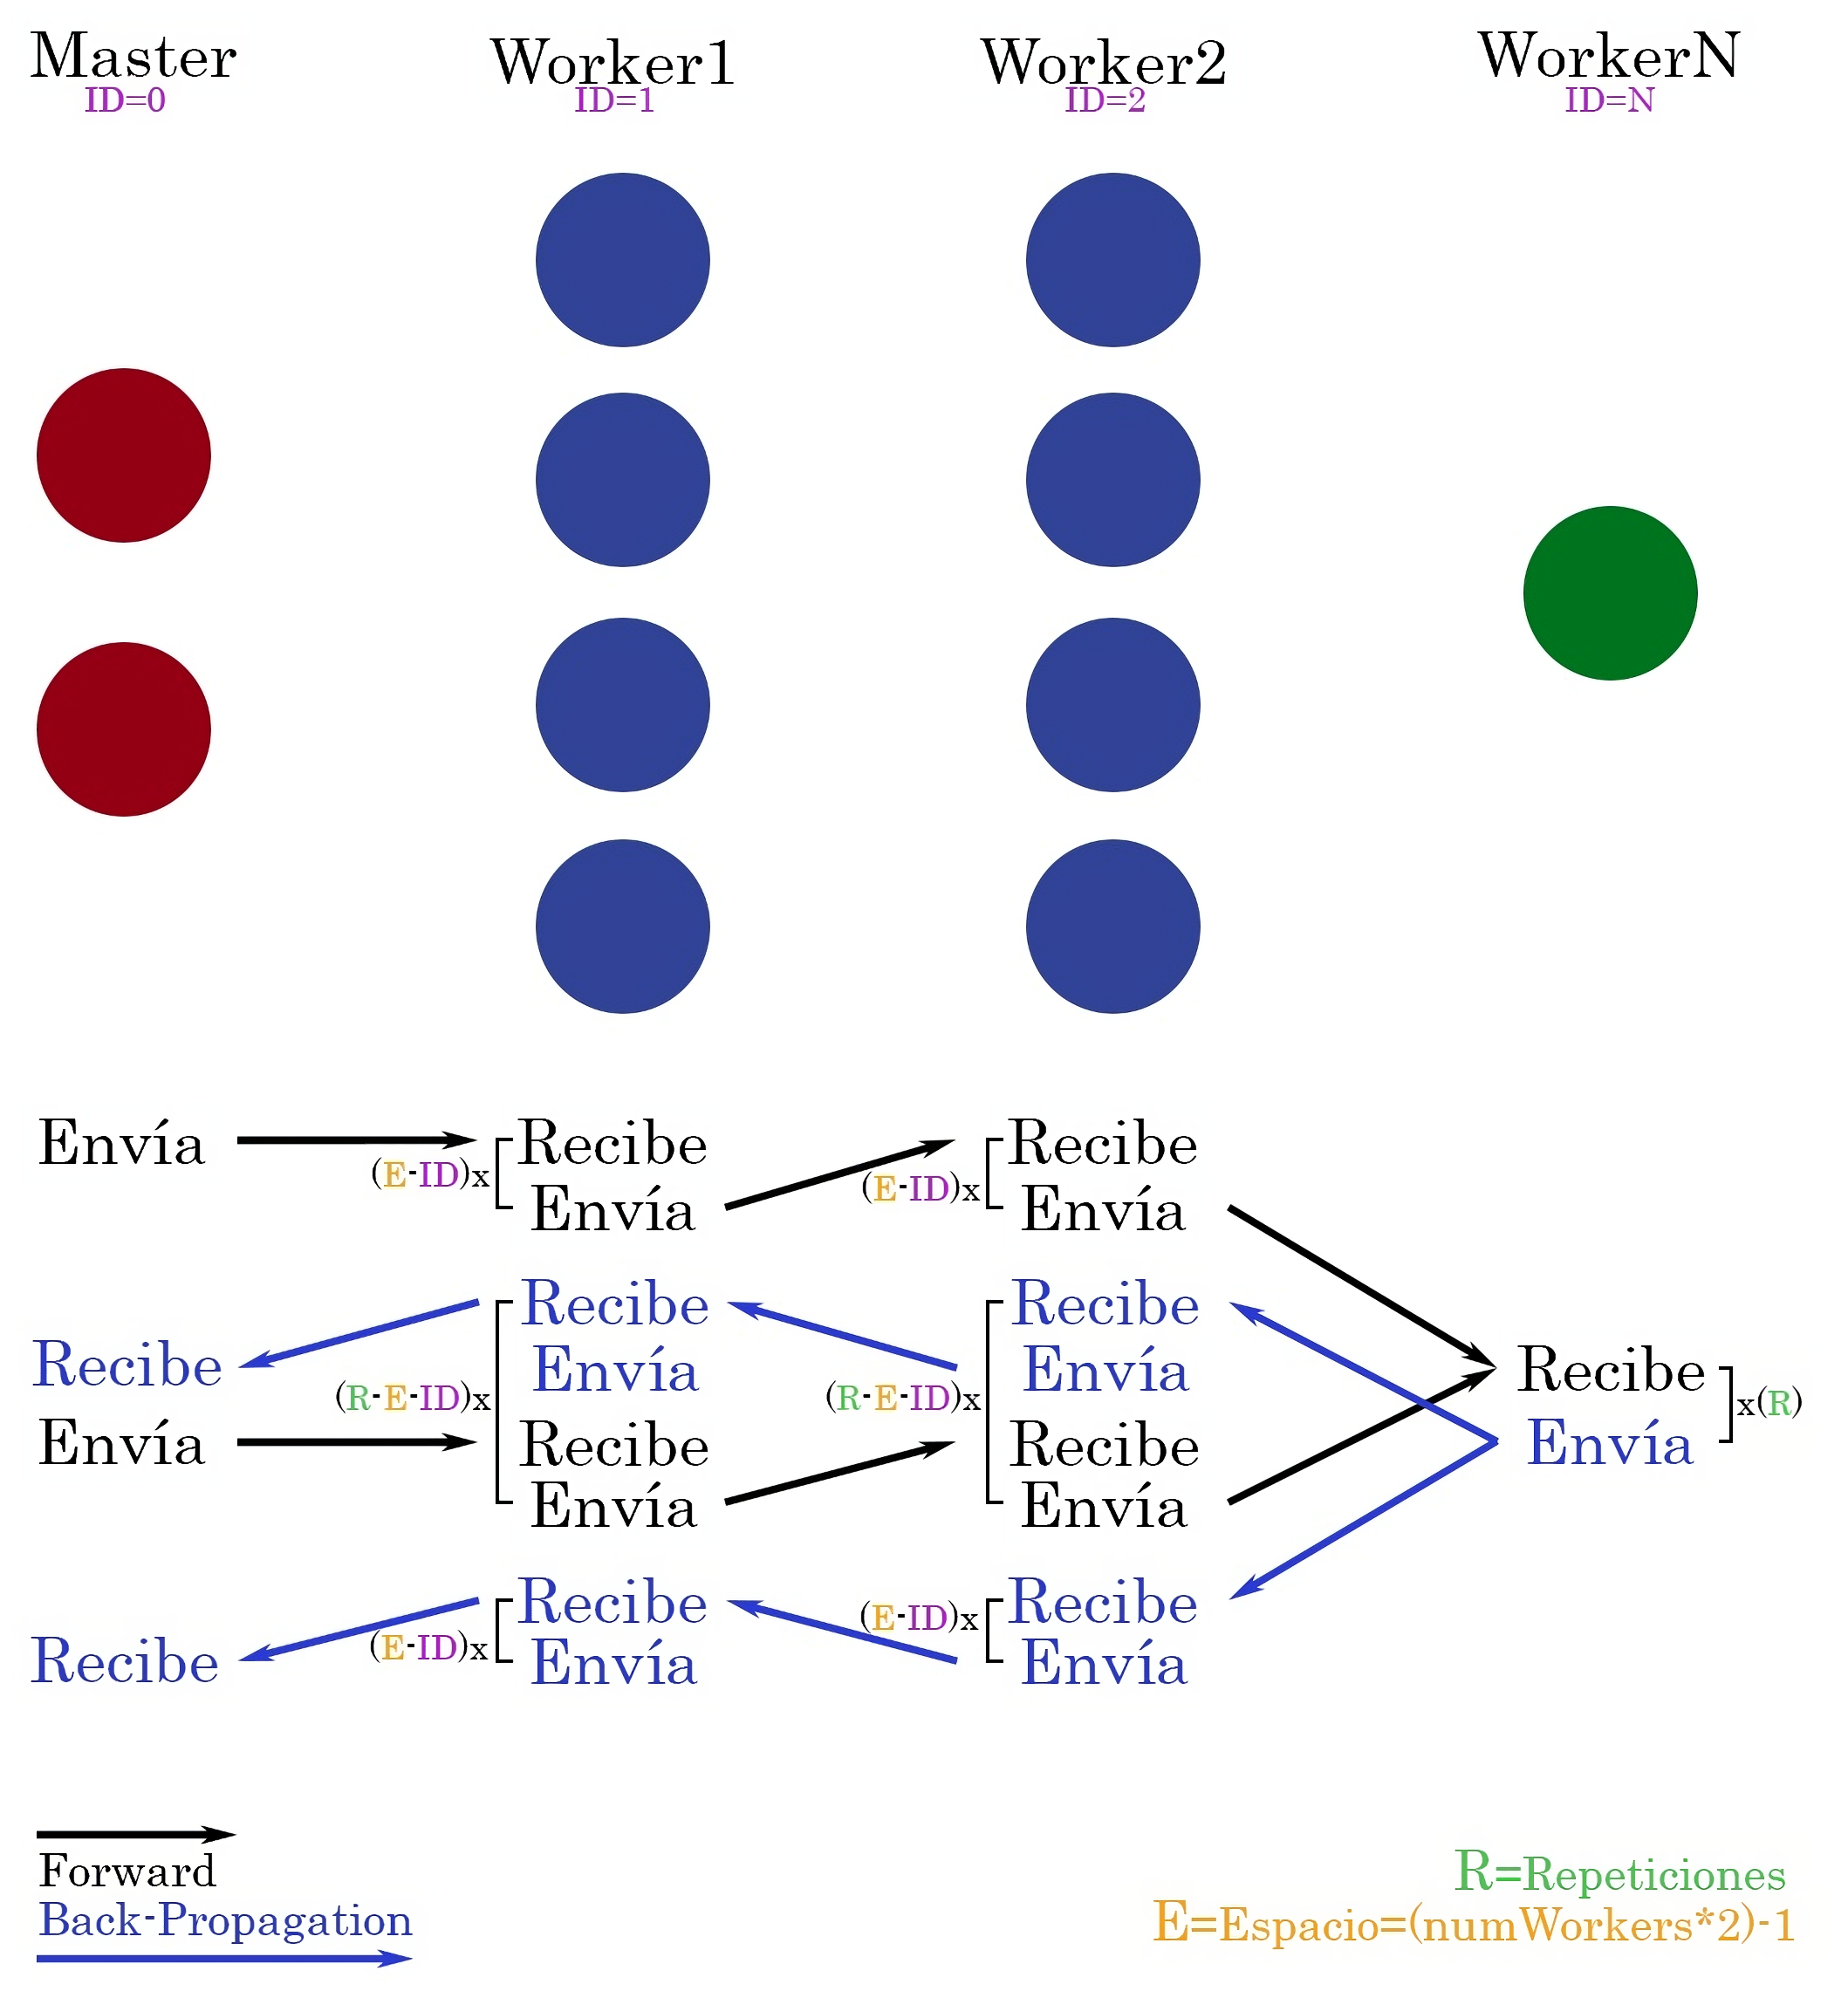
\includegraphics[width=0.55\textwidth]{images/chapter_3/redneu_mpi2}
		\caption{MPI - PipeLine Rede Neuronal}
		\label{fig:redneumpipipe}
	\end{figure}
	
	Al ser un proceso iterativo, en el cual el modelo va aprendiendo en la fase de entrenamiento, a primera vista, dividir la población entre procesos no parece ser beneficioso para el correcto aprendizaje de la red. Sin embargo, en redes neuronales hay un proceso llamado fine tuning \cite{malladi2023fine} que consiste en entrenar una red neuronal, con unos pesos ya calculados. Basándonos en esta técnica, podemos implementar una mejora en la cual dividamos la población inicial entre procesos, y en paralelo ejecutamos la fase de entrenamiento. Una vez finalizadas el master recibe los pesos de cada worker y hace la media. 
	
	Cuanto más grande sea la red neuronal mejor, tanto en rendimiento como en evaluación. En las redes neuronales grandes, un nodo se especializa en unos ciertos parámetros, por lo que no hay demasiadas intersecciones entre los entrenamientos de los procesos. Pero hay que dividir correctamente la población inicial entre los procesos. 
	
	\begin{enumerate}
		\item Con una población distinta, depende del tamaño de la red. 
		\begin{itemize}
			\item Si es una red pequeña, esta técnica no es muy efectiva. La diferencia de pesos entre procesos puede llegar a ser grande, y al hacer la media dar evaluaciones incorrectas. 		
			\item Sin embargo con muchas capas se mejora la evaluación. Cada proceso especializa unas neuronas y al juntarlas en el master no intersecan.			
		\end{itemize}		
		\item Si enviamos una población parecida, depende de la inicialización de los pesos, pero muy seguramente no surta efecto. Es como ejecutar varias veces el algoritmo en diferentes ejecuciones.
		
	\end{enumerate}	
	
	

	